% Options for packages loaded elsewhere
\PassOptionsToPackage{unicode}{hyperref}
\PassOptionsToPackage{hyphens}{url}
\PassOptionsToPackage{dvipsnames,svgnames,x11names}{xcolor}
%
\documentclass[
  ignorenonframetext,
  aspectratio=169]{beamer}
\usepackage{pgfpages}
\setbeamertemplate{caption}[numbered]
\setbeamertemplate{caption label separator}{: }
\setbeamercolor{caption name}{fg=normal text.fg}
\beamertemplatenavigationsymbolsempty
% Prevent slide breaks in the middle of a paragraph
\widowpenalties 1 10000
\raggedbottom
\setbeamertemplate{part page}{
  \centering
  \begin{beamercolorbox}[sep=16pt,center]{part title}
    \usebeamerfont{part title}\insertpart\par
  \end{beamercolorbox}
}
\setbeamertemplate{section page}{
  \centering
  \begin{beamercolorbox}[sep=12pt,center]{part title}
    \usebeamerfont{section title}\insertsection\par
  \end{beamercolorbox}
}
\setbeamertemplate{subsection page}{
  \centering
  \begin{beamercolorbox}[sep=8pt,center]{part title}
    \usebeamerfont{subsection title}\insertsubsection\par
  \end{beamercolorbox}
}
\AtBeginPart{
  \frame{\partpage}
}
\AtBeginSection{
  \ifbibliography
  \else
    \frame{\sectionpage}
  \fi
}
\AtBeginSubsection{
  \frame{\subsectionpage}
}
\usepackage{amsmath,amssymb}
\usepackage{iftex}
\ifPDFTeX
  \usepackage[T1]{fontenc}
  \usepackage[utf8]{inputenc}
  \usepackage{textcomp} % provide euro and other symbols
\else % if luatex or xetex
  \usepackage{unicode-math} % this also loads fontspec
  \defaultfontfeatures{Scale=MatchLowercase}
  \defaultfontfeatures[\rmfamily]{Ligatures=TeX,Scale=1}
\fi
\usepackage{lmodern}
\usecolortheme{lily}
\ifPDFTeX\else
  % xetex/luatex font selection
\fi
% Use upquote if available, for straight quotes in verbatim environments
\IfFileExists{upquote.sty}{\usepackage{upquote}}{}
\IfFileExists{microtype.sty}{% use microtype if available
  \usepackage[]{microtype}
  \UseMicrotypeSet[protrusion]{basicmath} % disable protrusion for tt fonts
}{}
\makeatletter
\@ifundefined{KOMAClassName}{% if non-KOMA class
  \IfFileExists{parskip.sty}{%
    \usepackage{parskip}
  }{% else
    \setlength{\parindent}{0pt}
    \setlength{\parskip}{6pt plus 2pt minus 1pt}}
}{% if KOMA class
  \KOMAoptions{parskip=half}}
\makeatother
\usepackage{xcolor}
\newif\ifbibliography
\usepackage{color}
\usepackage{fancyvrb}
\newcommand{\VerbBar}{|}
\newcommand{\VERB}{\Verb[commandchars=\\\{\}]}
\DefineVerbatimEnvironment{Highlighting}{Verbatim}{commandchars=\\\{\}}
% Add ',fontsize=\small' for more characters per line
\usepackage{framed}
\definecolor{shadecolor}{RGB}{248,248,248}
\newenvironment{Shaded}{\begin{snugshade}}{\end{snugshade}}
\newcommand{\AlertTok}[1]{\textcolor[rgb]{0.94,0.16,0.16}{#1}}
\newcommand{\AnnotationTok}[1]{\textcolor[rgb]{0.56,0.35,0.01}{\textbf{\textit{#1}}}}
\newcommand{\AttributeTok}[1]{\textcolor[rgb]{0.13,0.29,0.53}{#1}}
\newcommand{\BaseNTok}[1]{\textcolor[rgb]{0.00,0.00,0.81}{#1}}
\newcommand{\BuiltInTok}[1]{#1}
\newcommand{\CharTok}[1]{\textcolor[rgb]{0.31,0.60,0.02}{#1}}
\newcommand{\CommentTok}[1]{\textcolor[rgb]{0.56,0.35,0.01}{\textit{#1}}}
\newcommand{\CommentVarTok}[1]{\textcolor[rgb]{0.56,0.35,0.01}{\textbf{\textit{#1}}}}
\newcommand{\ConstantTok}[1]{\textcolor[rgb]{0.56,0.35,0.01}{#1}}
\newcommand{\ControlFlowTok}[1]{\textcolor[rgb]{0.13,0.29,0.53}{\textbf{#1}}}
\newcommand{\DataTypeTok}[1]{\textcolor[rgb]{0.13,0.29,0.53}{#1}}
\newcommand{\DecValTok}[1]{\textcolor[rgb]{0.00,0.00,0.81}{#1}}
\newcommand{\DocumentationTok}[1]{\textcolor[rgb]{0.56,0.35,0.01}{\textbf{\textit{#1}}}}
\newcommand{\ErrorTok}[1]{\textcolor[rgb]{0.64,0.00,0.00}{\textbf{#1}}}
\newcommand{\ExtensionTok}[1]{#1}
\newcommand{\FloatTok}[1]{\textcolor[rgb]{0.00,0.00,0.81}{#1}}
\newcommand{\FunctionTok}[1]{\textcolor[rgb]{0.13,0.29,0.53}{\textbf{#1}}}
\newcommand{\ImportTok}[1]{#1}
\newcommand{\InformationTok}[1]{\textcolor[rgb]{0.56,0.35,0.01}{\textbf{\textit{#1}}}}
\newcommand{\KeywordTok}[1]{\textcolor[rgb]{0.13,0.29,0.53}{\textbf{#1}}}
\newcommand{\NormalTok}[1]{#1}
\newcommand{\OperatorTok}[1]{\textcolor[rgb]{0.81,0.36,0.00}{\textbf{#1}}}
\newcommand{\OtherTok}[1]{\textcolor[rgb]{0.56,0.35,0.01}{#1}}
\newcommand{\PreprocessorTok}[1]{\textcolor[rgb]{0.56,0.35,0.01}{\textit{#1}}}
\newcommand{\RegionMarkerTok}[1]{#1}
\newcommand{\SpecialCharTok}[1]{\textcolor[rgb]{0.81,0.36,0.00}{\textbf{#1}}}
\newcommand{\SpecialStringTok}[1]{\textcolor[rgb]{0.31,0.60,0.02}{#1}}
\newcommand{\StringTok}[1]{\textcolor[rgb]{0.31,0.60,0.02}{#1}}
\newcommand{\VariableTok}[1]{\textcolor[rgb]{0.00,0.00,0.00}{#1}}
\newcommand{\VerbatimStringTok}[1]{\textcolor[rgb]{0.31,0.60,0.02}{#1}}
\newcommand{\WarningTok}[1]{\textcolor[rgb]{0.56,0.35,0.01}{\textbf{\textit{#1}}}}
\usepackage{graphicx}
\makeatletter
\def\maxwidth{\ifdim\Gin@nat@width>\linewidth\linewidth\else\Gin@nat@width\fi}
\def\maxheight{\ifdim\Gin@nat@height>\textheight\textheight\else\Gin@nat@height\fi}
\makeatother
% Scale images if necessary, so that they will not overflow the page
% margins by default, and it is still possible to overwrite the defaults
% using explicit options in \includegraphics[width, height, ...]{}
\setkeys{Gin}{width=\maxwidth,height=\maxheight,keepaspectratio}
% Set default figure placement to htbp
\makeatletter
\def\fps@figure{htbp}
\makeatother
\usepackage{soul}
\setlength{\emergencystretch}{3em} % prevent overfull lines
\providecommand{\tightlist}{%
  \setlength{\itemsep}{0pt}\setlength{\parskip}{0pt}}
\setcounter{secnumdepth}{-\maxdimen} % remove section numbering
\definecolor{darkturquoise}{rgb}{0.0, 0.81, 0.82}
\useinnertheme{circles}
\let\oldShaded\Shaded %Change fontsize of R code chunks
\let\endoldShaded\endShaded
\renewenvironment{Shaded}{\scriptsize\oldShaded}{\endoldShaded}
\let\oldverbatim\verbatim %Change fontsize of code chunk output
\let\endoldverbatim\endverbatim
\renewenvironment{verbatim}{\tiny\oldverbatim}{\endoldverbatim}
\ifLuaTeX
  \usepackage{selnolig}  % disable illegal ligatures
\fi
\IfFileExists{bookmark.sty}{\usepackage{bookmark}}{\usepackage{hyperref}}
\IfFileExists{xurl.sty}{\usepackage{xurl}}{} % add URL line breaks if available
\urlstyle{same}
\hypersetup{
  pdftitle={Linear models},
  pdfauthor={Samuel Robinson, Ph.D.},
  colorlinks=true,
  linkcolor={Maroon},
  filecolor={Maroon},
  citecolor={Blue},
  urlcolor={blue},
  pdfcreator={LaTeX via pandoc}}

\title{Linear models}
\subtitle{Modeling\ldots{} linearly!}
\author{Samuel Robinson, Ph.D.}
\date{Sep.~22, 2023}

\begin{document}
\frame{\titlepage}

\hypertarget{part-1-how-do-they-work}{%
\section{Part 1: How do they work?}\label{part-1-how-do-they-work}}

\begin{frame}{Outline}
\protect\hypertarget{outline}{}
\begin{columns}[T]
\begin{column}{0.48\textwidth}
\begin{itemize}[<+->]
\item
  What are linear models? How do I fit them?
\item
  Making sure the model is working properly
\item
  Plotting and interpreting model results
\end{itemize}
\end{column}

\begin{column}{0.48\textwidth}
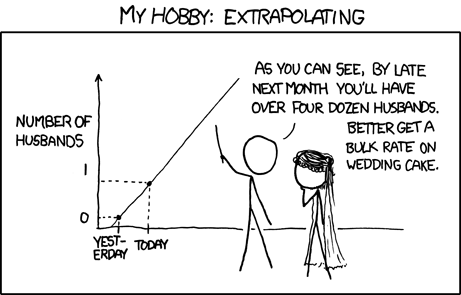
\includegraphics[width=1\textwidth,height=\textheight]{xkcd_extrapolating.png}
\end{column}
\end{columns}
\end{frame}

\begin{frame}{Motivation}
\protect\hypertarget{motivation}{}
\begin{itemize}
\tightlist
\item
  \emph{I measured 2 things and I want to know if they're related to
  each other}
\end{itemize}

\begin{itemize}
\tightlist
\item
  \emph{I have groups of data, and I want to know whether the means are
  different}
\end{itemize}

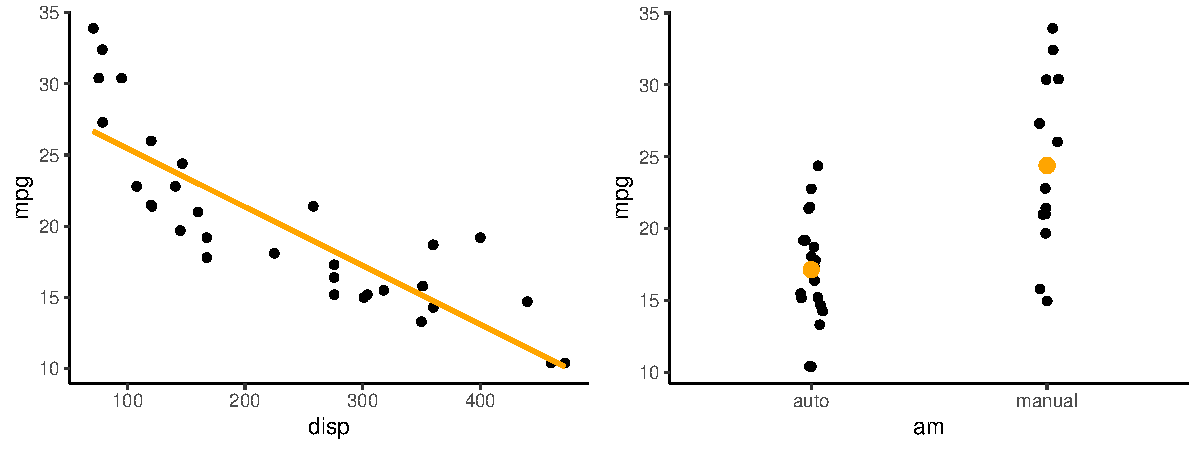
\includegraphics{03-Lecture_files/figure-beamer/examplePlots-1.pdf}
\end{frame}

\begin{frame}{Terminology}
\protect\hypertarget{terminology}{}
Linear models go by many different names. All these models are all doing
\emph{exactly the same thing}:

\begin{itemize}[<+->]
\item
  Linear regression
\item
  Least-squares regression
\item
  Simple linear model (SLM)
\item
  Multiple linear model/regression
\item
  Analysis of Variance (ANOVA)
\item
  Analysis of Covariance (ANCOVA)
\end{itemize}

\pause

I use a set of terminology that I find very helpful, from
\href{https://link.springer.com/chapter/10.1007/978-94-011-5430-7_3}{Berliner
(1996)}. I'll be using it here, as well as for describing more complex
models.
\end{frame}

\begin{frame}{Model terminology}
\protect\hypertarget{model-terminology}{}
All linear models take the form: \begin{equation*} 
\begin{split}
\textcolor{orange}{\hat{y}} & = \textcolor{blue}{b_0} + \textcolor{blue}{b_1}\textcolor{darkturquoise}{x_1} + \textcolor{blue}{b_2}\textcolor{darkturquoise}{x_2} ... + \textcolor{blue}{b_i}\textcolor{darkturquoise}{x_i} \\
y & \sim Normal(\textcolor{orange}{\hat{y}},\textcolor{red}{\sigma})
\end{split}
\end{equation*}

\pause

\begin{itemize}[<+->]
\tightlist
\item
  \(y\) is the thing you're interested in predicting
\item
  \(\textcolor{orange}{\hat{y}}\) is the \emph{predicted value} of \(y\)
\item
  \(\textcolor{darkturquoise}{x_1...x_i}\) are \emph{predictors} of
  \emph{y}
\item
  \(\textcolor{blue}{b_1...b_i}\) are \emph{coefficients} for each
  predictor \(\textcolor{darkturquoise}{x_i}\)
\item
  \(\textcolor{blue}{b_0}\) is the \emph{intercept}, a coefficient that
  doesn't depend on predictors
\item
  \(y\sim Normal(\textcolor{orange}{\hat{y}},\textcolor{red}{\sigma})\)
  means:

  \begin{itemize}[<+->]
  \tightlist
  \item
    ``\(y\) follows a Normal distribution with mean
    \(\textcolor{orange}{\hat{y}}\) and SD \(\textcolor{red}{\sigma}\)''
  \end{itemize}
\end{itemize}

\pause

This may look terrifying, but let's use a simple example:
\end{frame}

\begin{frame}{Example}
\protect\hypertarget{example}{}
\begin{columns}[T]
\begin{column}{0.48\textwidth}
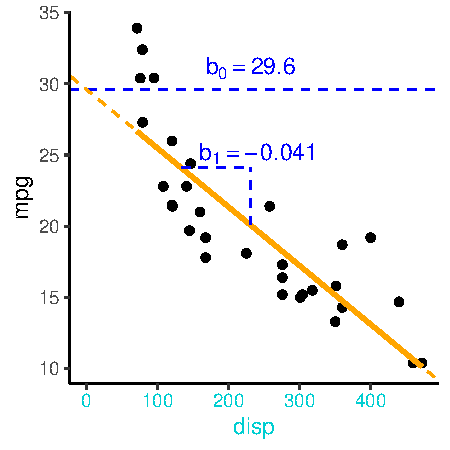
\includegraphics{03-Lecture_files/figure-beamer/unnamed-chunk-1-1.pdf}

\begin{equation*} 
\begin{split}
\textcolor{orange}{\hat{mpg}} & = \textcolor{blue}{b_0} + \textcolor{blue}{b_1}\textcolor{darkturquoise}{disp} \\
mpg & \sim Normal(\textcolor{orange}{\hat{mpg}},\textcolor{red}{\sigma})
\end{split}
\end{equation*}
\end{column}

\begin{column}{0.48\textwidth}
\begin{itemize}[<+->]
\tightlist
\item
  \(mpg\) is the thing you're interested in predicting
\item
  \(\textcolor{orange}{\hat{mpg}}\) is the \emph{predicted value} of
  \(mpg\)
\item
  \(\textcolor{darkturquoise}{disp}\) is the \emph{predictor} of
  \emph{mpg}
\item
  \(\textcolor{blue}{b_0}\) is the \emph{intercept},
  \(\textcolor{blue}{b_1}\) is the \emph{coefficient} (slope) for
  \(\textcolor{darkturquoise}{disp}\)
\item
  \(mpg\sim Normal(\textcolor{orange}{\hat{mpg}},\textcolor{red}{\sigma})\)
  means:

  \begin{itemize}[<+->]
  \tightlist
  \item
    ``\(mpg\) follows a Normal distribution with mean
    \(\textcolor{orange}{\hat{mpg}}\) and SD
    \(\textcolor{red}{\sigma}\)''
  \end{itemize}
\item
  \(\textcolor{red}{\sigma}\) isn't displayed on the figure. Where is
  it?
\end{itemize}
\end{column}
\end{columns}
\end{frame}

\begin{frame}{Example (cont.)}
\protect\hypertarget{example-cont.}{}
\(\textcolor{red}{\sigma}\) isn't displayed on the figure. Where is it?

\begin{columns}[T]
\begin{column}{0.48\textwidth}
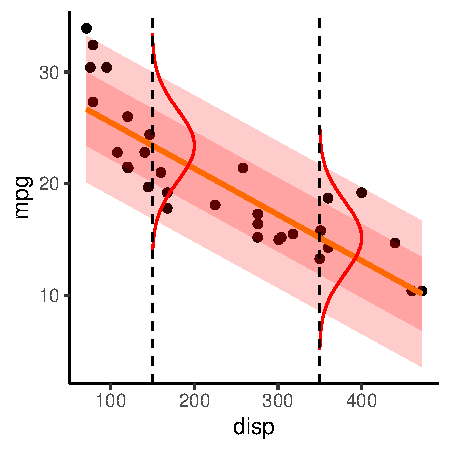
\includegraphics{03-Lecture_files/figure-beamer/unnamed-chunk-2-1.pdf}
\end{column}

\begin{column}{0.48\textwidth}
\begin{itemize}[<+->]
\tightlist
\item
  \(\textcolor{red}{\sigma}\) is the ``leftover'' or ``residual''
  variance
\item
  i.e.~variation between samples that the model couldn't explain
\item
  Since
  \(y\sim Normal(\textcolor{orange}{\hat{y}},\textcolor{red}{\sigma})\),
  this means that points are normally distributed around the
  \emph{entire line} of \(\textcolor{orange}{\hat{y}}\)
\item
  If you took a vertical slice at each part of the x-axis, the
  distribution would be \emph{Normal}
\end{itemize}
\end{column}
\end{columns}
\end{frame}

\begin{frame}[fragile]{How do I get R to fit this model?}
\protect\hypertarget{how-do-i-get-r-to-fit-this-model}{}
\texttt{lm} is one of the main functions used for linear modeling:

\begin{Shaded}
\begin{Highlighting}[]
\CommentTok{\#Formula= y \textasciitilde{} x, data = Name of the dataframe containing mpg \& disp}
\NormalTok{mod1 }\OtherTok{\textless{}{-}} \FunctionTok{lm}\NormalTok{(mpg }\SpecialCharTok{\textasciitilde{}}\NormalTok{ disp, }\AttributeTok{data =}\NormalTok{ mtcars); }\FunctionTok{summary}\NormalTok{(mod1)}
\end{Highlighting}
\end{Shaded}

\begin{verbatim}
## 
## Call:
## lm(formula = mpg ~ disp, data = mtcars)
## 
## Residuals:
##     Min      1Q  Median      3Q     Max 
## -4.8922 -2.2022 -0.9631  1.6272  7.2305 
## 
## Coefficients:
##              Estimate Std. Error t value Pr(>|t|)    
## (Intercept) 29.599855   1.229720  24.070  < 2e-16 ***
## disp        -0.041215   0.004712  -8.747 9.38e-10 ***
## ---
## Signif. codes:  0 '***' 0.001 '**' 0.01 '*' 0.05 '.' 0.1 ' ' 1
## 
## Residual standard error: 3.251 on 30 degrees of freedom
## Multiple R-squared:  0.7183, Adjusted R-squared:  0.709 
## F-statistic: 76.51 on 1 and 30 DF,  p-value: 9.38e-10
\end{verbatim}

For a detailed breakdown of \texttt{lm}'s output, click
\href{https://stats.stackexchange.com/questions/5135/interpretation-of-rs-lm-output}{here}
\end{frame}

\begin{frame}[fragile]{Simulate data}
\protect\hypertarget{simulate-data}{}
Now that we know how linear models work, we can simulate our own data:

\begin{columns}[T]
\begin{column}{0.5\textwidth}
\scriptsize

\begin{Shaded}
\begin{Highlighting}[]
\CommentTok{\#Parameters:}

\NormalTok{b0 }\OtherTok{\textless{}{-}} \DecValTok{1} \CommentTok{\#Intercept}
\NormalTok{b1 }\OtherTok{\textless{}{-}} \DecValTok{2} \CommentTok{\#Slope }
\NormalTok{sigma }\OtherTok{\textless{}{-}} \DecValTok{3} \CommentTok{\#SD}

\CommentTok{\#Make up some data:}

\NormalTok{x }\OtherTok{\textless{}{-}} \DecValTok{0}\SpecialCharTok{:}\DecValTok{30} \CommentTok{\#Predictor values}

\CommentTok{\#Predicted y values}
\NormalTok{pred\_y }\OtherTok{\textless{}{-}}\NormalTok{ b0 }\SpecialCharTok{+}\NormalTok{ b1}\SpecialCharTok{*}\NormalTok{x }

\CommentTok{\#Add "noise" around pred\_y}
\NormalTok{actual\_y }\OtherTok{\textless{}{-}} \FunctionTok{rnorm}\NormalTok{(}\AttributeTok{n =} \FunctionTok{length}\NormalTok{(pred\_y),}
                  \AttributeTok{mean =}\NormalTok{ pred\_y,}
                  \AttributeTok{sd=}\NormalTok{ sigma)}
\end{Highlighting}
\end{Shaded}
\end{column}

\begin{column}{0.5\textwidth}
\scriptsize

\begin{Shaded}
\begin{Highlighting}[]
\CommentTok{\#Plot the data we just made}
\FunctionTok{plot}\NormalTok{(x,pred\_y,}\AttributeTok{col=}\StringTok{\textquotesingle{}orange\textquotesingle{}}\NormalTok{,}\AttributeTok{pch=}\DecValTok{19}\NormalTok{,}\AttributeTok{type=}\StringTok{\textquotesingle{}l\textquotesingle{}}\NormalTok{,}
     \AttributeTok{ylab=}\StringTok{\textquotesingle{}y\textquotesingle{}}\NormalTok{) }
\FunctionTok{points}\NormalTok{(x,actual\_y,}\AttributeTok{col=}\StringTok{\textquotesingle{}black\textquotesingle{}}\NormalTok{,}\AttributeTok{pch=}\DecValTok{19}\NormalTok{)}
\end{Highlighting}
\end{Shaded}

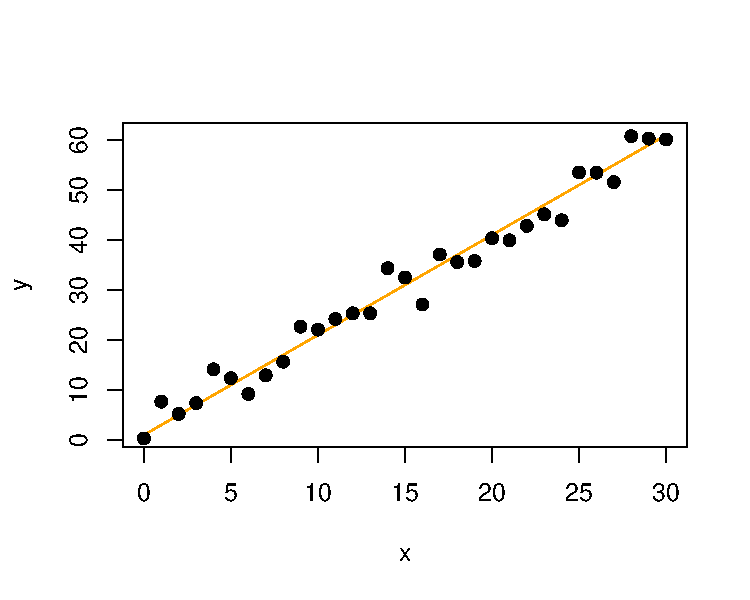
\includegraphics{03-Lecture_files/figure-beamer/unnamed-chunk-5-1.pdf}
\end{column}
\end{columns}
\end{frame}

\begin{frame}[fragile]{Fit a model from simulated data}
\protect\hypertarget{fit-a-model-from-simulated-data}{}
How does R do at finding the coefficients? Remember:
\(b_0 = 1, b_1 = 2, \sigma = 3\)

\begin{Shaded}
\begin{Highlighting}[]
\NormalTok{fakeDat }\OtherTok{\textless{}{-}} \FunctionTok{data.frame}\NormalTok{(}\AttributeTok{x =}\NormalTok{ x, }\AttributeTok{y =}\NormalTok{ actual\_y, }\AttributeTok{pred =}\NormalTok{ pred\_y) }\CommentTok{\#Simulated data in a dataframe }
\NormalTok{mod1sim }\OtherTok{\textless{}{-}} \FunctionTok{lm}\NormalTok{(y }\SpecialCharTok{\textasciitilde{}}\NormalTok{ x, }\AttributeTok{data =}\NormalTok{ fakeDat); }\FunctionTok{summary}\NormalTok{(mod1sim) }\CommentTok{\#Fit model}
\end{Highlighting}
\end{Shaded}

\begin{verbatim}
## 
## Call:
## lm(formula = y ~ x, data = fakeDat)
## 
## Residuals:
##     Min      1Q  Median      3Q     Max 
## -5.7568 -1.7623 -0.2176  1.9419  5.3572 
## 
## Coefficients:
##             Estimate Std. Error t value Pr(>|t|)    
## (Intercept)  2.02974    1.00445   2.021   0.0526 .  
## x            1.92670    0.05751  33.499   <2e-16 ***
## ---
## Signif. codes:  0 '***' 0.001 '**' 0.01 '*' 0.05 '.' 0.1 ' ' 1
## 
## Residual standard error: 2.864 on 29 degrees of freedom
## Multiple R-squared:  0.9748, Adjusted R-squared:  0.9739 
## F-statistic:  1122 on 1 and 29 DF,  p-value: < 2.2e-16
\end{verbatim}

\pause

Modeling philosophy: all models are approximating a \textbf{generative
process}.

\emph{It is up to us to think about what this process might be like.}
\end{frame}

\begin{frame}{What about categorical data?}
\protect\hypertarget{what-about-categorical-data}{}
\begin{columns}[T]
\begin{column}{0.48\textwidth}
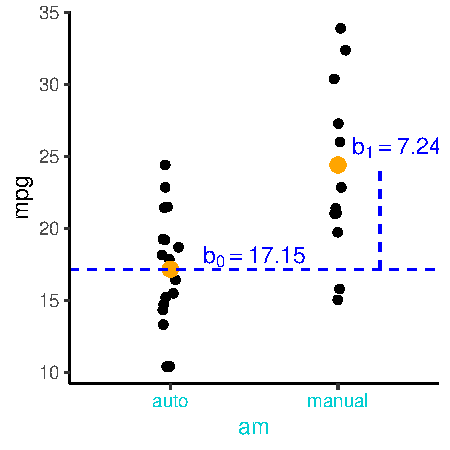
\includegraphics{03-Lecture_files/figure-beamer/unnamed-chunk-7-1.pdf}

\begin{equation*} 
\begin{split}
\textcolor{orange}{\hat{mpg}} & = \textcolor{blue}{b_0} + \textcolor{blue}{b_1}\textcolor{darkturquoise}{am} \\
mpg & \sim Normal(\textcolor{orange}{\hat{mpg}},\textcolor{red}{\sigma})
\end{split}
\end{equation*}
\end{column}

\begin{column}{0.48\textwidth}
This uses \emph{exactly the same} math!

\begin{itemize}[<+->]
\tightlist
\item
  \(mpg\) is the thing you're interested in predicting
\item
  \(\textcolor{orange}{\hat{mpg}}\) is the \emph{predicted value} of
  \(mpg\)
\item
  \(\textcolor{darkturquoise}{am}\) is the \emph{predictor} of
  \emph{mpg}

  \begin{itemize}[<+->]
  \tightlist
  \item
    set of 0s and 1s, not continuous
  \end{itemize}
\item
  \(\textcolor{blue}{b_0}\) is the \emph{intercept},
  \(\textcolor{blue}{b_1}\) is the \emph{coefficient} for
  \(\textcolor{darkturquoise}{am}\)
\item
  Where is \(\textcolor{red}{\sigma}\)?
\end{itemize}
\end{column}
\end{columns}
\end{frame}

\begin{frame}[fragile]{How do I get R to fit this model?}
\protect\hypertarget{how-do-i-get-r-to-fit-this-model-1}{}
Syntax is exactly the same for this model

\tiny

\begin{Shaded}
\begin{Highlighting}[]
\CommentTok{\#Formula structure: y \textasciitilde{} x}
\NormalTok{mod2 }\OtherTok{\textless{}{-}} \FunctionTok{lm}\NormalTok{(mpg }\SpecialCharTok{\textasciitilde{}}\NormalTok{ am, }\CommentTok{\#mpg depends on am}
           \AttributeTok{data =}\NormalTok{ mtcars) }\CommentTok{\#Name of the dataframe containing mpg \& am}
\FunctionTok{summary}\NormalTok{(mod2)}
\end{Highlighting}
\end{Shaded}

\begin{verbatim}
## 
## Call:
## lm(formula = mpg ~ am, data = mtcars)
## 
## Residuals:
##     Min      1Q  Median      3Q     Max 
## -9.3923 -3.0923 -0.2974  3.2439  9.5077 
## 
## Coefficients:
##             Estimate Std. Error t value Pr(>|t|)    
## (Intercept)   17.147      1.125  15.247 1.13e-15 ***
## am             7.245      1.764   4.106 0.000285 ***
## ---
## Signif. codes:  0 '***' 0.001 '**' 0.01 '*' 0.05 '.' 0.1 ' ' 1
## 
## Residual standard error: 4.902 on 30 degrees of freedom
## Multiple R-squared:  0.3598, Adjusted R-squared:  0.3385 
## F-statistic: 16.86 on 1 and 30 DF,  p-value: 0.000285
\end{verbatim}
\end{frame}

\begin{frame}[fragile]{A challenger approaches!}
\protect\hypertarget{a-challenger-approaches}{}
\begin{itemize}[<+->]
\tightlist
\item
  Simulate your own data with 2 discrete levels. My suggestion:

  \begin{itemize}[<+->]
  \tightlist
  \item
    \st{Steal}Borrow my code, and change the predictor from continuous
    to discrete
  \item
    Useful command: \texttt{rep} (replicate)

    \begin{itemize}[<+->]
    \tightlist
    \item
      e.g.~\texttt{rep(x=c(0,1),each=10)}
    \end{itemize}
  \item
    Useful command: \texttt{rnorm} (generate normally-distributed data)

    \begin{itemize}[<+->]
    \tightlist
    \item
      e.g.~\texttt{rnorm(n=100,mean=0,sd=1)}
    \end{itemize}
  \end{itemize}
\item
  Use \texttt{lm} to fit a model to the data you just simulated

  \begin{itemize}[<+->]
  \tightlist
  \item
    How does R do at guessing your coefficients?
  \end{itemize}
\end{itemize}
\end{frame}

\hypertarget{part-2-more-bells-and-whistles}{%
\section{Part 2: More bells and
whistles}\label{part-2-more-bells-and-whistles}}

\begin{frame}{Motivation}
\protect\hypertarget{motivation-1}{}
\begin{itemize}
\tightlist
\item
  \emph{I have 2+ groups of data, and I want to know whether the means
  are different}
\end{itemize}

\begin{itemize}
\tightlist
\item
  \emph{I have 2+ groups of bivariate data, and I want to know whether
  the relationships differ between groups}
\end{itemize}

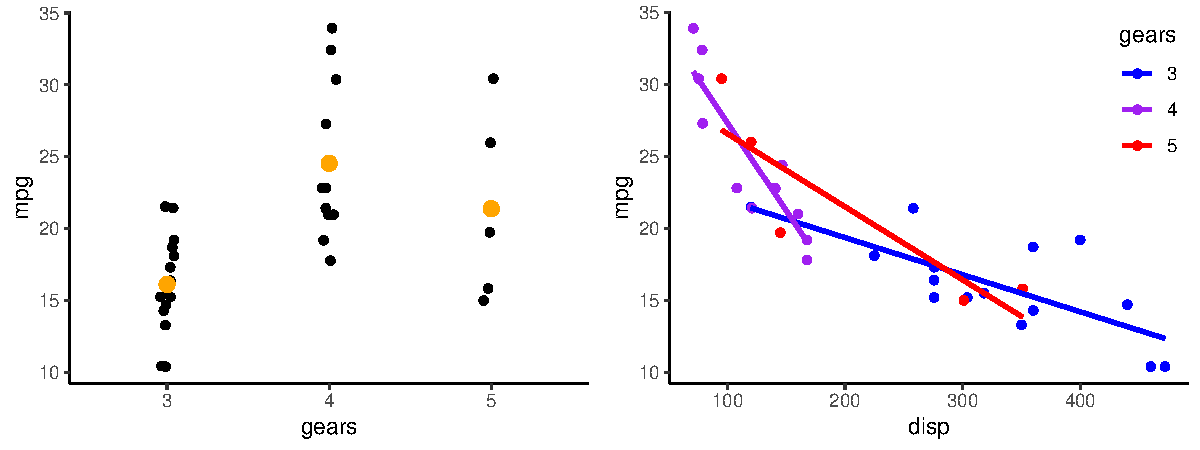
\includegraphics{03-Lecture_files/figure-beamer/examplePlots2-1.pdf}
\end{frame}

\begin{frame}{Categorial data, 3 categories}
\protect\hypertarget{categorial-data-3-categories}{}
\begin{columns}[T]
\begin{column}{0.48\textwidth}
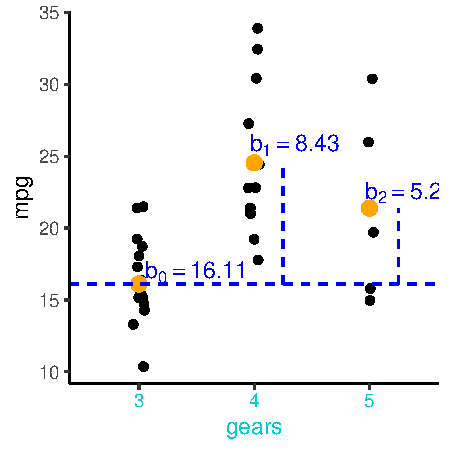
\includegraphics{03-Lecture_files/figure-beamer/unnamed-chunk-9-1.pdf}

\begin{equation*} 
\begin{split}
\textcolor{orange}{\hat{mpg}} & = \textcolor{blue}{b_0} + \textcolor{blue}{b_1}\textcolor{darkturquoise}{gears_4} + \textcolor{blue}{b_2}\textcolor{darkturquoise}{gears_5} \\
mpg & \sim Normal(\textcolor{orange}{\hat{mpg}},\textcolor{red}{\sigma})
\end{split}
\end{equation*}
\end{column}

\begin{column}{0.48\textwidth}
The more factor levels, the more coefficients:

\begin{itemize}
\tightlist
\item
  \(mpg\) is the thing you're interested in predicting
\item
  \(\textcolor{orange}{\hat{mpg}}\) is the \emph{predicted value} of
  \(mpg\)
\item
  \(\textcolor{darkturquoise}{gear}\) is the \emph{predictor} of
  \emph{mpg}
\item
  set of 0s and 1s
\item
  \(\textcolor{darkturquoise}{gears_4}=\) ``is this data point from a
  4-gear car?''
\item
  \(\textcolor{blue}{b_0}=\) \emph{intercept}
\item
  \([\textcolor{blue}{b_1},\textcolor{blue}{b_2}]=\) are
  \emph{coefficients} for \(\textcolor{darkturquoise}{gears}\)
\end{itemize}
\end{column}
\end{columns}
\end{frame}

\begin{frame}[fragile]{How do I get R to fit this model?}
\protect\hypertarget{how-do-i-get-r-to-fit-this-model-2}{}
\tiny

\begin{Shaded}
\begin{Highlighting}[]
\CommentTok{\#Formula structure: y \textasciitilde{} x}
\NormalTok{mod1 }\OtherTok{\textless{}{-}} \FunctionTok{lm}\NormalTok{(mpg }\SpecialCharTok{\textasciitilde{}} \FunctionTok{factor}\NormalTok{(gear), }\CommentTok{\#mpg depends on gears}
           \AttributeTok{data =}\NormalTok{ mtcars) }\CommentTok{\#Name of the dataframe containing mpg \& gears}
\FunctionTok{summary}\NormalTok{(mod1)}
\end{Highlighting}
\end{Shaded}

\begin{verbatim}
## 
## Call:
## lm(formula = mpg ~ factor(gear), data = mtcars)
## 
## Residuals:
##     Min      1Q  Median      3Q     Max 
## -6.7333 -3.2333 -0.9067  2.8483  9.3667 
## 
## Coefficients:
##               Estimate Std. Error t value Pr(>|t|)    
## (Intercept)     16.107      1.216  13.250 7.87e-14 ***
## factor(gear)4    8.427      1.823   4.621 7.26e-05 ***
## factor(gear)5    5.273      2.431   2.169   0.0384 *  
## ---
## Signif. codes:  0 '***' 0.001 '**' 0.01 '*' 0.05 '.' 0.1 ' ' 1
## 
## Residual standard error: 4.708 on 29 degrees of freedom
## Multiple R-squared:  0.4292, Adjusted R-squared:  0.3898 
## F-statistic:  10.9 on 2 and 29 DF,  p-value: 0.0002948
\end{verbatim}
\end{frame}

\begin{frame}[fragile]{Dummy variables}
\protect\hypertarget{dummy-variables}{}
\tiny

\begin{Shaded}
\begin{Highlighting}[]
\NormalTok{mod1Matrix }\OtherTok{\textless{}{-}} \FunctionTok{model.matrix}\NormalTok{(mod1) }\CommentTok{\#Get model matrix (columns used to predict mpg)}
\FunctionTok{head}\NormalTok{(mod1Matrix,}\DecValTok{28}\NormalTok{) }\CommentTok{\#Show first 28 rows of model matrix}
\end{Highlighting}
\end{Shaded}

\begin{verbatim}
##                     (Intercept) factor(gear)4 factor(gear)5
## Mazda RX4                     1             1             0
## Mazda RX4 Wag                 1             1             0
## Datsun 710                    1             1             0
## Hornet 4 Drive                1             0             0
## Hornet Sportabout             1             0             0
## Valiant                       1             0             0
## Duster 360                    1             0             0
## Merc 240D                     1             1             0
## Merc 230                      1             1             0
## Merc 280                      1             1             0
## Merc 280C                     1             1             0
## Merc 450SE                    1             0             0
## Merc 450SL                    1             0             0
## Merc 450SLC                   1             0             0
## Cadillac Fleetwood            1             0             0
## Lincoln Continental           1             0             0
## Chrysler Imperial             1             0             0
## Fiat 128                      1             1             0
## Honda Civic                   1             1             0
## Toyota Corolla                1             1             0
## Toyota Corona                 1             0             0
## Dodge Challenger              1             0             0
## AMC Javelin                   1             0             0
## Camaro Z28                    1             0             0
## Pontiac Firebird              1             0             0
## Fiat X1-9                     1             1             0
## Porsche 914-2                 1             0             1
## Lotus Europa                  1             0             1
\end{verbatim}
\end{frame}

\begin{frame}{What about if 2 things are both important?}
\protect\hypertarget{what-about-if-2-things-are-both-important}{}
\begin{columns}[T]
\begin{column}{0.48\textwidth}
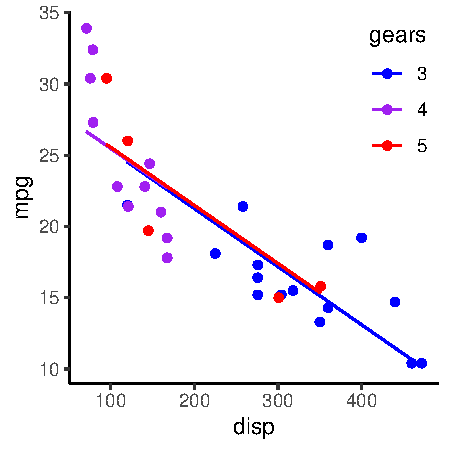
\includegraphics{03-Lecture_files/figure-beamer/unnamed-chunk-12-1.pdf}

\begin{equation*} 
\begin{split}
\textcolor{orange}{\hat{mpg}} & = \textcolor{blue}{b_0} + \textcolor{blue}{b_1}\textcolor{darkturquoise}{disp} \\
&+ \textcolor{blue}{b_2}\textcolor{darkturquoise}{gears_4} + \textcolor{blue}{b_3}\textcolor{darkturquoise}{gears_5} \\
mpg & \sim Normal(\textcolor{orange}{\hat{mpg}},\textcolor{red}{\sigma})
\end{split}
\end{equation*}
\end{column}

\begin{column}{0.48\textwidth}
\begin{itemize}
\tightlist
\item
  Suppose that both \(\textcolor{darkturquoise}{disp}\) and
  \(\textcolor{darkturquoise}{gears}\) are important for predicting
  \(mpg\)?
\item
  This is very similar to the last example, except that now we've added
  \(\textcolor{darkturquoise}{disp}\)
\item
  \(\textcolor{darkturquoise}{gears}\) now changes the intercept, while
  \(\textcolor{darkturquoise}{disp}\) changes the slope of all the lines
\item
  Does it look like \(\textcolor{darkturquoise}{gear}\) is very
  important?
\end{itemize}
\end{column}
\end{columns}
\end{frame}

\begin{frame}[fragile]{How do I get R to fit this model?}
\protect\hypertarget{how-do-i-get-r-to-fit-this-model-3}{}
\tiny

\begin{Shaded}
\begin{Highlighting}[]
\CommentTok{\#mpg depends on disp and gears}
\NormalTok{mod2 }\OtherTok{\textless{}{-}} \FunctionTok{lm}\NormalTok{(mpg }\SpecialCharTok{\textasciitilde{}}\NormalTok{ disp}\SpecialCharTok{+}\FunctionTok{factor}\NormalTok{(gear), }\AttributeTok{data =}\NormalTok{ mtcars) }
\FunctionTok{summary}\NormalTok{(mod2)}
\end{Highlighting}
\end{Shaded}

\begin{verbatim}
## 
## Call:
## lm(formula = mpg ~ disp + factor(gear), data = mtcars)
## 
## Residuals:
##     Min      1Q  Median      3Q     Max 
## -4.9155 -2.1892 -0.9054  1.5790  7.2498 
## 
## Coefficients:
##                Estimate Std. Error t value Pr(>|t|)    
## (Intercept)   29.411183   2.627966  11.192 7.58e-12 ***
## disp          -0.040774   0.007601  -5.364 1.03e-05 ***
## factor(gear)4  0.138017   2.021332   0.068    0.946    
## factor(gear)5  0.224712   1.976090   0.114    0.910    
## ---
## Signif. codes:  0 '***' 0.001 '**' 0.01 '*' 0.05 '.' 0.1 ' ' 1
## 
## Residual standard error: 3.365 on 28 degrees of freedom
## Multiple R-squared:  0.7185, Adjusted R-squared:  0.6883 
## F-statistic: 23.82 on 3 and 28 DF,  p-value: 7.31e-08
\end{verbatim}
\end{frame}

\begin{frame}[fragile]{Dummy variables}
\protect\hypertarget{dummy-variables-1}{}
\tiny

\begin{Shaded}
\begin{Highlighting}[]
\NormalTok{mod2Matrix }\OtherTok{\textless{}{-}} \FunctionTok{model.matrix}\NormalTok{(mod2) }\CommentTok{\#Get model matrix (columns used to predict mpg)}
\FunctionTok{colnames}\NormalTok{(mod2Matrix) }\OtherTok{\textless{}{-}} \FunctionTok{gsub}\NormalTok{(}\StringTok{\textquotesingle{}factor}\SpecialCharTok{\textbackslash{}\textbackslash{}}\StringTok{(gear}\SpecialCharTok{\textbackslash{}\textbackslash{}}\StringTok{)\textquotesingle{}}\NormalTok{,}\StringTok{\textquotesingle{}gear\textquotesingle{}}\NormalTok{,}\FunctionTok{colnames}\NormalTok{(mod2Matrix)) }\CommentTok{\#Shorten colnames}
\FunctionTok{head}\NormalTok{(mod2Matrix,}\DecValTok{28}\NormalTok{) }\CommentTok{\#Show first 28 rows of model matrix}
\end{Highlighting}
\end{Shaded}

\begin{verbatim}
##                     (Intercept)  disp gear4 gear5
## Mazda RX4                     1 160.0     1     0
## Mazda RX4 Wag                 1 160.0     1     0
## Datsun 710                    1 108.0     1     0
## Hornet 4 Drive                1 258.0     0     0
## Hornet Sportabout             1 360.0     0     0
## Valiant                       1 225.0     0     0
## Duster 360                    1 360.0     0     0
## Merc 240D                     1 146.7     1     0
## Merc 230                      1 140.8     1     0
## Merc 280                      1 167.6     1     0
## Merc 280C                     1 167.6     1     0
## Merc 450SE                    1 275.8     0     0
## Merc 450SL                    1 275.8     0     0
## Merc 450SLC                   1 275.8     0     0
## Cadillac Fleetwood            1 472.0     0     0
## Lincoln Continental           1 460.0     0     0
## Chrysler Imperial             1 440.0     0     0
## Fiat 128                      1  78.7     1     0
## Honda Civic                   1  75.7     1     0
## Toyota Corolla                1  71.1     1     0
## Toyota Corona                 1 120.1     0     0
## Dodge Challenger              1 318.0     0     0
## AMC Javelin                   1 304.0     0     0
## Camaro Z28                    1 350.0     0     0
## Pontiac Firebird              1 400.0     0     0
## Fiat X1-9                     1  79.0     1     0
## Porsche 914-2                 1 120.3     0     1
## Lotus Europa                  1  95.1     0     1
\end{verbatim}
\end{frame}

\begin{frame}[fragile]{Interlude: problems with plotting raw data}
\protect\hypertarget{interlude-problems-with-plotting-raw-data}{}
\begin{itemize}
\tightlist
\item
  Say that I've fit the following model:\\
  \texttt{mpg\ \textasciitilde{}\ disp\ +\ factor(gear)}
\item
  All of the plots below are using raw data, but which one is ``telling
  the truth''?
\item
  Answer: \textbf{c}. \emph{a} and \emph{b} are hiding the effect of the
  other variable
\end{itemize}

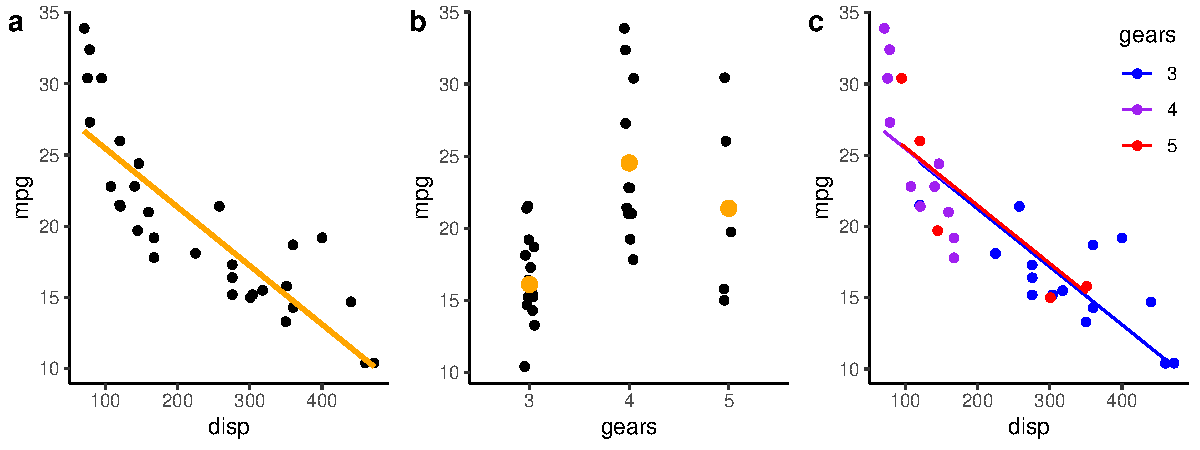
\includegraphics{03-Lecture_files/figure-beamer/unnamed-chunk-15-1.pdf}
\end{frame}

\begin{frame}[fragile]{How do I plot these model results?}
\protect\hypertarget{how-do-i-plot-these-model-results}{}
\begin{columns}[T]
\begin{column}{0.48\textwidth}
Rule for plotting model results:

\begin{enumerate}[<+->]
\tightlist
\item
  If the model uses \texttt{N} variables, you should show all \texttt{N}
  effects \emph{simultaneously}
\item
  If this is impractical, you should use a \textbf{partial effects plot}
\end{enumerate}

Other names for partial effects:

\begin{itemize}[<+->]
\tightlist
\item
  \emph{counterfactual} plot, \emph{predictor effect} plot,
  \emph{leverage} plot
\item
  Try using \texttt{effects} or \texttt{ggeffects}. Requires the
  \texttt{effects} and \texttt{ggeffect} packages
\end{itemize}
\end{column}

\begin{column}{0.48\textwidth}
Incorrect example, using raw data: \tiny

\begin{Shaded}
\begin{Highlighting}[]
\CommentTok{\#Fit model with 5 variables (all important)}
\NormalTok{simMod }\OtherTok{\textless{}{-}} \FunctionTok{lm}\NormalTok{(y}\SpecialCharTok{\textasciitilde{}}\NormalTok{X1}\SpecialCharTok{+}\NormalTok{X2}\SpecialCharTok{+}\NormalTok{X3}\SpecialCharTok{+}\NormalTok{X4}\SpecialCharTok{+}\NormalTok{X5,}\AttributeTok{data=}\NormalTok{pred) }
\CommentTok{\#Incorrect way, using raw data }
\FunctionTok{plot}\NormalTok{(y}\SpecialCharTok{\textasciitilde{}}\NormalTok{X5,}\AttributeTok{data=}\NormalTok{pred,}\AttributeTok{pch=}\DecValTok{19}\NormalTok{,}\AttributeTok{cex.lab=}\DecValTok{3}\NormalTok{) }
\end{Highlighting}
\end{Shaded}

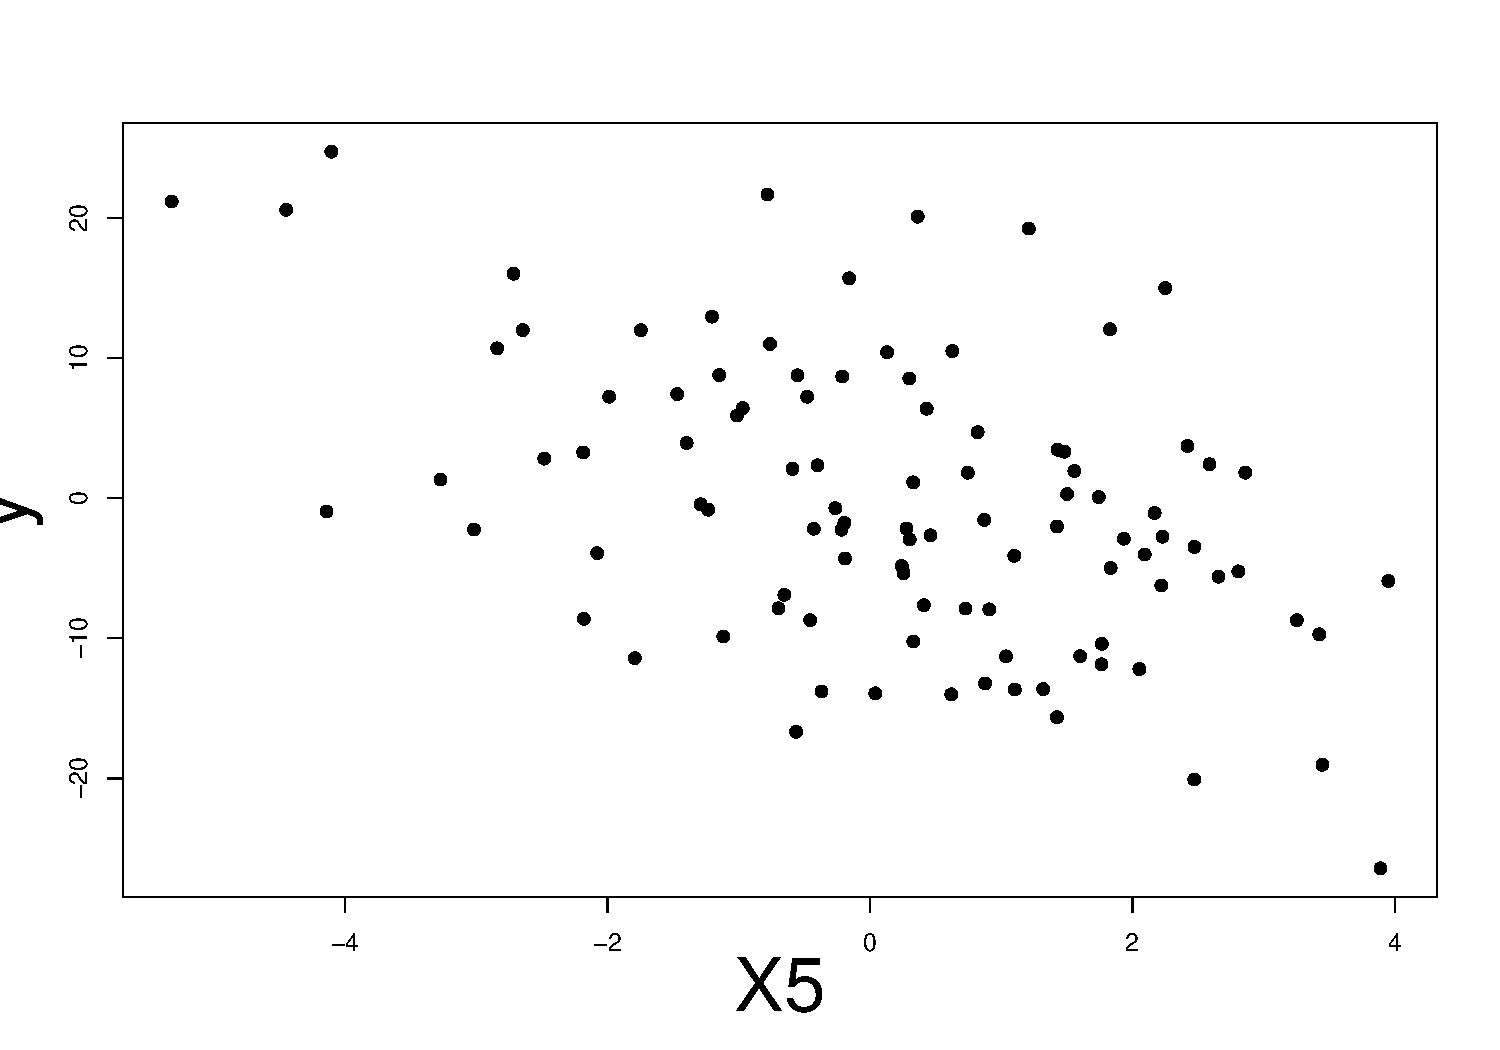
\includegraphics{03-Lecture_files/figure-beamer/unnamed-chunk-17-1.pdf}

\normalsize

The effect of \emph{X5} is actually \textbf{very} strong (\(p<0.0001\)),
but it doesn't look like it from this plot!
\end{column}
\end{columns}
\end{frame}

\begin{frame}[fragile]{Partial effects plots - using \emph{effects}}
\protect\hypertarget{partial-effects-plots---using-effects}{}
\tiny

\begin{Shaded}
\begin{Highlighting}[]
\FunctionTok{library}\NormalTok{(effects) }\CommentTok{\#Load effects package}
\NormalTok{simModEff }\OtherTok{\textless{}{-}} \FunctionTok{predictorEffects}\NormalTok{(simMod,}\AttributeTok{partial.residuals=}\ConstantTok{TRUE}\NormalTok{) }\CommentTok{\#Calculate partial effects}
\CommentTok{\#Plot partial effects}
\FunctionTok{plot}\NormalTok{(simModEff,}\AttributeTok{lines=}\FunctionTok{list}\NormalTok{(}\AttributeTok{col=}\StringTok{\textquotesingle{}red\textquotesingle{}}\NormalTok{), }\AttributeTok{partial.residuals=}\FunctionTok{list}\NormalTok{(}\AttributeTok{pch=}\DecValTok{19}\NormalTok{,}\AttributeTok{col=}\StringTok{\textquotesingle{}black\textquotesingle{}}\NormalTok{,}\AttributeTok{cex=}\FloatTok{0.25}\NormalTok{))}
\end{Highlighting}
\end{Shaded}

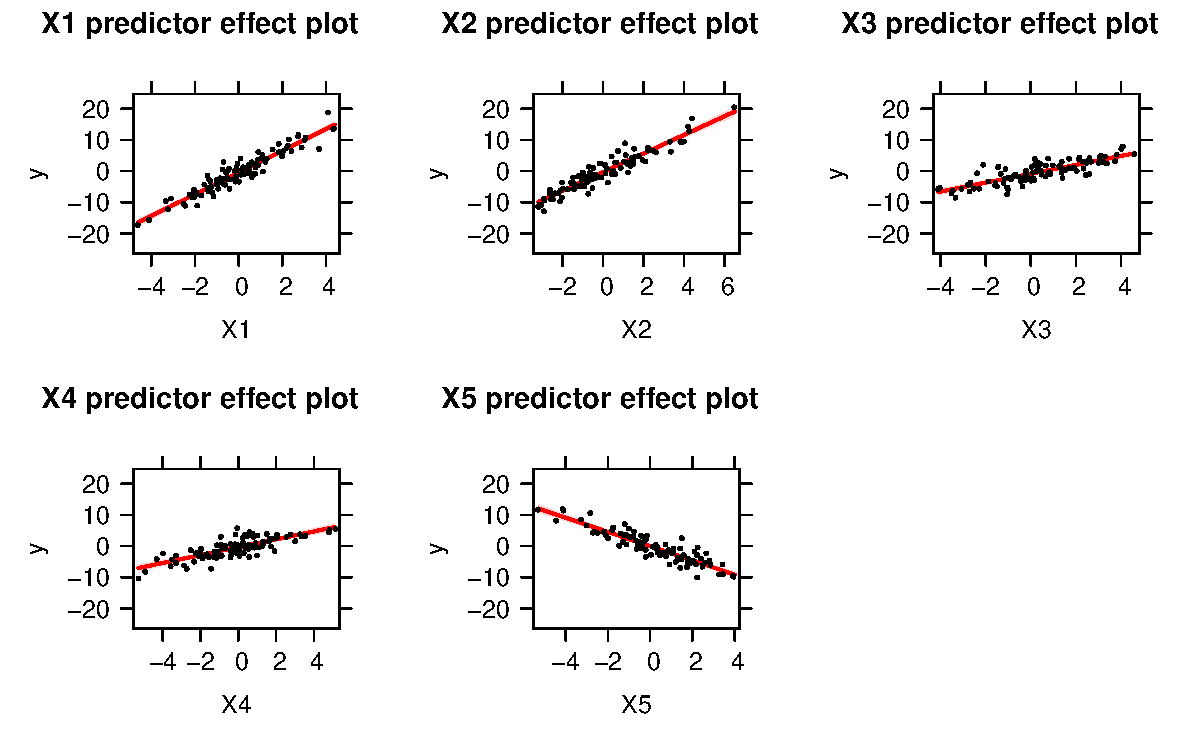
\includegraphics{03-Lecture_files/figure-beamer/unnamed-chunk-18-1.pdf}
\end{frame}

\begin{frame}[fragile]{Partial effects plots - using \emph{ggpredict}}
\protect\hypertarget{partial-effects-plots---using-ggpredict}{}
\tiny

\begin{Shaded}
\begin{Highlighting}[]
\FunctionTok{library}\NormalTok{(ggeffects) }\CommentTok{\#Load ggeffects package}
\NormalTok{simModEff2 }\OtherTok{\textless{}{-}} \FunctionTok{ggeffect}\NormalTok{(simMod,}\AttributeTok{terms=}\FunctionTok{c}\NormalTok{(}\StringTok{\textquotesingle{}X5\textquotesingle{}}\NormalTok{)) }\CommentTok{\#Calculate partial effects for X5}
\FunctionTok{plot}\NormalTok{(simModEff2) }\CommentTok{\#Plot effect of X5}
\end{Highlighting}
\end{Shaded}

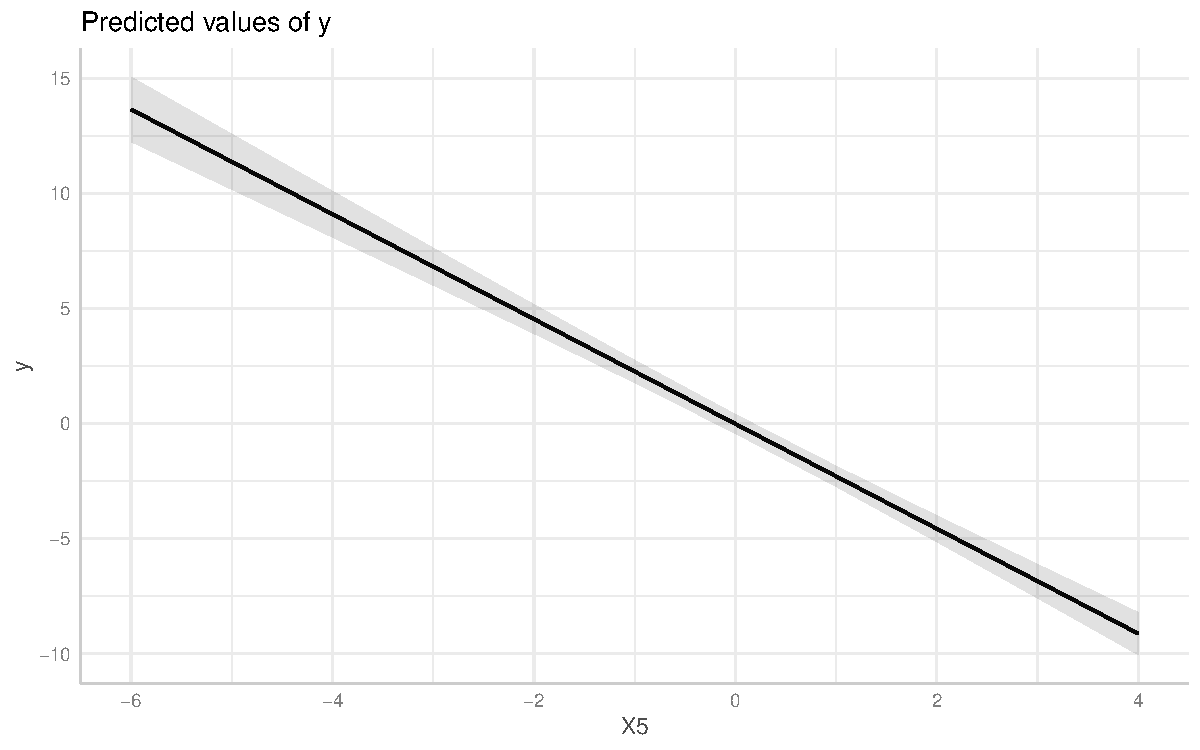
\includegraphics{03-Lecture_files/figure-beamer/unnamed-chunk-19-1.pdf}
\end{frame}

\begin{frame}{Interactions}
\protect\hypertarget{interactions}{}
What if the slopes \emph{and} intercepts differ between groups?

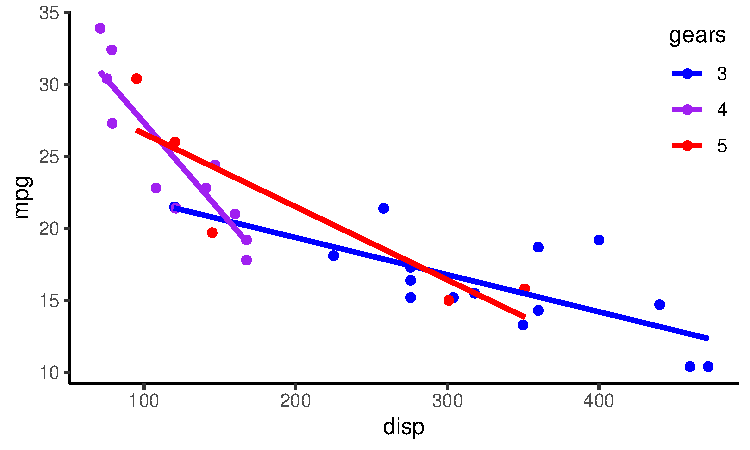
\includegraphics{03-Lecture_files/figure-beamer/unnamed-chunk-20-1.pdf}
\end{frame}

\begin{frame}{Interactions}
\protect\hypertarget{interactions-1}{}
\begin{columns}[T]
\begin{column}{0.48\textwidth}
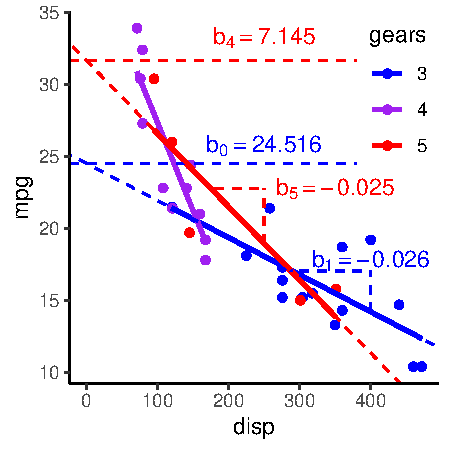
\includegraphics{03-Lecture_files/figure-beamer/unnamed-chunk-21-1.pdf}
\end{column}

\begin{column}{0.48\textwidth}
\begin{equation*} 
\begin{split}
\textcolor{orange}{\hat{mpg}} & = \textcolor{blue}{b_0} + \textcolor{blue}{b_1}\textcolor{darkturquoise}{disp}\\
& + \textcolor{blue}{b_2}\textcolor{darkturquoise}{gears_4} + \textcolor{blue}{b_3}\textcolor{darkturquoise}{gears_5}\\
& + \textcolor{blue}{b_4}\textcolor{darkturquoise}{(disp\times gears_4)}\\
& + \textcolor{blue}{b_5}\textcolor{darkturquoise}{(disp\times gears_5)}\\
mpg & \sim Normal(\textcolor{orange}{\hat{mpg}},\textcolor{red}{\sigma})
\end{split}
\end{equation*}

\begin{itemize}
\tightlist
\item
  Interactions occur when predictors are \emph{multiplied}
\item
  In this case, \(\textcolor{darkturquoise}{disp}\) is multiplied by
  \(\textcolor{darkturquoise}{gears_4}\) and
  \(\textcolor{darkturquoise}{gears_5}\)
\item
  \(\textcolor{darkturquoise}{gears}\) now changes the intercept and the
  slope of the relationship between \(mpg\) and
  \(\textcolor{darkturquoise}{disp}\)
\end{itemize}
\end{column}
\end{columns}
\end{frame}

\begin{frame}[fragile]{How do I get R to fit this model?}
\protect\hypertarget{how-do-i-get-r-to-fit-this-model-4}{}
\tiny

\begin{Shaded}
\begin{Highlighting}[]
\CommentTok{\#mpg depends on disp interacted (*) with gears}
\NormalTok{mod2 }\OtherTok{\textless{}{-}} \FunctionTok{lm}\NormalTok{(mpg }\SpecialCharTok{\textasciitilde{}}\NormalTok{ disp}\SpecialCharTok{*}\FunctionTok{factor}\NormalTok{(gear), }\AttributeTok{data =}\NormalTok{ mtcars) }
\FunctionTok{summary}\NormalTok{(mod2)}
\end{Highlighting}
\end{Shaded}

\begin{verbatim}
## 
## Call:
## lm(formula = mpg ~ disp * factor(gear), data = mtcars)
## 
## Residuals:
##     Min      1Q  Median      3Q     Max 
## -4.5986 -1.5990 -0.0143  1.6329  4.9926 
## 
## Coefficients:
##                     Estimate Std. Error t value Pr(>|t|)    
## (Intercept)        24.515566   2.462431   9.956 2.32e-10 ***
## disp               -0.025770   0.007265  -3.547 0.001505 ** 
## factor(gear)4      15.051963   3.558043   4.230 0.000256 ***
## factor(gear)5       7.145380   3.535913   2.021 0.053711 .  
## disp:factor(gear)4 -0.096442   0.021261  -4.536 0.000114 ***
## disp:factor(gear)5 -0.025005   0.013320  -1.877 0.071742 .  
## ---
## Signif. codes:  0 '***' 0.001 '**' 0.01 '*' 0.05 '.' 0.1 ' ' 1
## 
## Residual standard error: 2.579 on 26 degrees of freedom
## Multiple R-squared:  0.8465, Adjusted R-squared:  0.817 
## F-statistic: 28.67 on 5 and 26 DF,  p-value: 8.452e-10
\end{verbatim}

\small

Beware of fitting too many interactions, or else the \emph{Bilbo effect}
occurs!
\end{frame}

\begin{frame}[fragile]{Dummy variables}
\protect\hypertarget{dummy-variables-2}{}
\tiny

\begin{Shaded}
\begin{Highlighting}[]
\NormalTok{mod2Matrix }\OtherTok{\textless{}{-}} \FunctionTok{model.matrix}\NormalTok{(mod2) }\CommentTok{\#Get model matrix (columns used to predict mpg)}
\FunctionTok{colnames}\NormalTok{(mod2Matrix) }\OtherTok{\textless{}{-}} \FunctionTok{gsub}\NormalTok{(}\StringTok{\textquotesingle{}factor}\SpecialCharTok{\textbackslash{}\textbackslash{}}\StringTok{(gear}\SpecialCharTok{\textbackslash{}\textbackslash{}}\StringTok{)\textquotesingle{}}\NormalTok{,}\StringTok{\textquotesingle{}gear\textquotesingle{}}\NormalTok{,}\FunctionTok{colnames}\NormalTok{(mod2Matrix)) }\CommentTok{\#Shorten colnames}
\FunctionTok{head}\NormalTok{(mod2Matrix,}\DecValTok{28}\NormalTok{) }\CommentTok{\#Show first 28 rows of model matrix}
\end{Highlighting}
\end{Shaded}

\begin{verbatim}
##                     (Intercept)  disp gear4 gear5 disp:gear4 disp:gear5
## Mazda RX4                     1 160.0     1     0      160.0        0.0
## Mazda RX4 Wag                 1 160.0     1     0      160.0        0.0
## Datsun 710                    1 108.0     1     0      108.0        0.0
## Hornet 4 Drive                1 258.0     0     0        0.0        0.0
## Hornet Sportabout             1 360.0     0     0        0.0        0.0
## Valiant                       1 225.0     0     0        0.0        0.0
## Duster 360                    1 360.0     0     0        0.0        0.0
## Merc 240D                     1 146.7     1     0      146.7        0.0
## Merc 230                      1 140.8     1     0      140.8        0.0
## Merc 280                      1 167.6     1     0      167.6        0.0
## Merc 280C                     1 167.6     1     0      167.6        0.0
## Merc 450SE                    1 275.8     0     0        0.0        0.0
## Merc 450SL                    1 275.8     0     0        0.0        0.0
## Merc 450SLC                   1 275.8     0     0        0.0        0.0
## Cadillac Fleetwood            1 472.0     0     0        0.0        0.0
## Lincoln Continental           1 460.0     0     0        0.0        0.0
## Chrysler Imperial             1 440.0     0     0        0.0        0.0
## Fiat 128                      1  78.7     1     0       78.7        0.0
## Honda Civic                   1  75.7     1     0       75.7        0.0
## Toyota Corolla                1  71.1     1     0       71.1        0.0
## Toyota Corona                 1 120.1     0     0        0.0        0.0
## Dodge Challenger              1 318.0     0     0        0.0        0.0
## AMC Javelin                   1 304.0     0     0        0.0        0.0
## Camaro Z28                    1 350.0     0     0        0.0        0.0
## Pontiac Firebird              1 400.0     0     0        0.0        0.0
## Fiat X1-9                     1  79.0     1     0       79.0        0.0
## Porsche 914-2                 1 120.3     0     1        0.0      120.3
## Lotus Europa                  1  95.1     0     1        0.0       95.1
\end{verbatim}
\end{frame}

\begin{frame}[fragile]{A challenger approaches!}
\protect\hypertarget{a-challenger-approaches-1}{}
\begin{itemize}[<+->]
\tightlist
\item
  Since you're all bat folks, here's some bat data!

  \begin{itemize}[<+->]
  \tightlist
  \item
    \texttt{batDat.csv}
  \end{itemize}
\item
  Data: 100 bat weights from 2 cities, recorded along with sex and age
\item
  How do these variables affect bat weight?

  \begin{itemize}[<+->]
  \tightlist
  \item
    Think about how these variables might be related to weight using
    your \texttt{brain}
  \item
    Fit a model using \texttt{lm}
  \item
    Make some plots, using \texttt{effects} or \texttt{ggeffects}
  \end{itemize}
\end{itemize}
\end{frame}

\hypertarget{part-3-models-behaving-badly}{%
\section{Part 3: Models behaving
badly}\label{part-3-models-behaving-badly}}

\begin{frame}{Motivation}
\protect\hypertarget{motivation-2}{}
Are my model results reliable?

\begin{itemize}[<+->]
\tightlist
\item
  Residual checks
\item
  Transformations
\item
  Collinearity
\item
  How much stuff should I put into my model?
\end{itemize}
\end{frame}

\begin{frame}{Assumptions of linear regression}
\protect\hypertarget{assumptions-of-linear-regression}{}
\begin{columns}[T]
\begin{column}{0.48\textwidth}
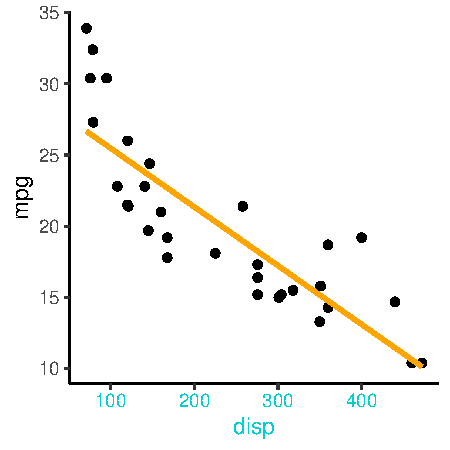
\includegraphics{03-Lecture_files/figure-beamer/unnamed-chunk-24-1.pdf}

\begin{equation*} 
\begin{split}
\textcolor{orange}{\hat{mpg}} & = \textcolor{blue}{b_0} + \textcolor{blue}{b_1}\textcolor{darkturquoise}{disp} \\
mpg & \sim Normal(\textcolor{orange}{\hat{mpg}},\textcolor{red}{\sigma})
\end{split}
\end{equation*}
\end{column}

\begin{column}{0.48\textwidth}
There are 3 main assumptions to this model:

\begin{enumerate}[<+->]
\tightlist
\item
  The relationship between \(\textcolor{darkturquoise}{disp}\) and
  \(mpg\) is linear
\item
  \(mpg\) (the data) is Normally distributed around
  \(\textcolor{orange}{\hat{mpg}}\) (the line)
\item
  \(\textcolor{red}{\sigma}\) is the same everywhere
\end{enumerate}

This is pretty easy to see if you only have 1 variable, but\ldots{}
\end{column}
\end{columns}
\end{frame}

\begin{frame}{What if I have many variables?}
\protect\hypertarget{what-if-i-have-many-variables}{}
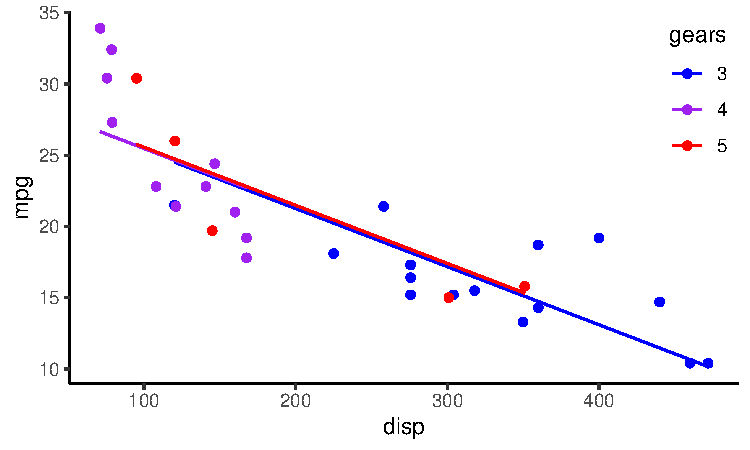
\includegraphics{03-Lecture_files/figure-beamer/unnamed-chunk-25-1.pdf}

Difficult to see if the assumptions are met
\end{frame}

\begin{frame}[fragile]{Solution: residual checks}
\protect\hypertarget{solution-residual-checks}{}
Some common ways of checking the assumptions: \textbf{residual plots}

\tiny

\begin{Shaded}
\begin{Highlighting}[]
\NormalTok{mod1 }\OtherTok{\textless{}{-}} \FunctionTok{lm}\NormalTok{(mpg}\SpecialCharTok{\textasciitilde{}}\NormalTok{disp}\SpecialCharTok{*}\FunctionTok{factor}\NormalTok{(gear),}\AttributeTok{data=}\NormalTok{mtcars) }\CommentTok{\#Fits model}
\FunctionTok{par}\NormalTok{(}\AttributeTok{mfrow=}\FunctionTok{c}\NormalTok{(}\DecValTok{1}\NormalTok{,}\DecValTok{2}\NormalTok{),}\AttributeTok{mar=}\FunctionTok{c}\NormalTok{(}\DecValTok{3}\NormalTok{,}\DecValTok{3}\NormalTok{,}\DecValTok{1}\NormalTok{,}\DecValTok{1}\NormalTok{)}\SpecialCharTok{+}\DecValTok{1}\NormalTok{) }\CommentTok{\#Splits plot into 2}
\FunctionTok{plot}\NormalTok{(mod1, }\AttributeTok{which=}\FunctionTok{c}\NormalTok{(}\DecValTok{1}\NormalTok{,}\DecValTok{2}\NormalTok{)) }\CommentTok{\#1st and 2nd residual plots}
\end{Highlighting}
\end{Shaded}

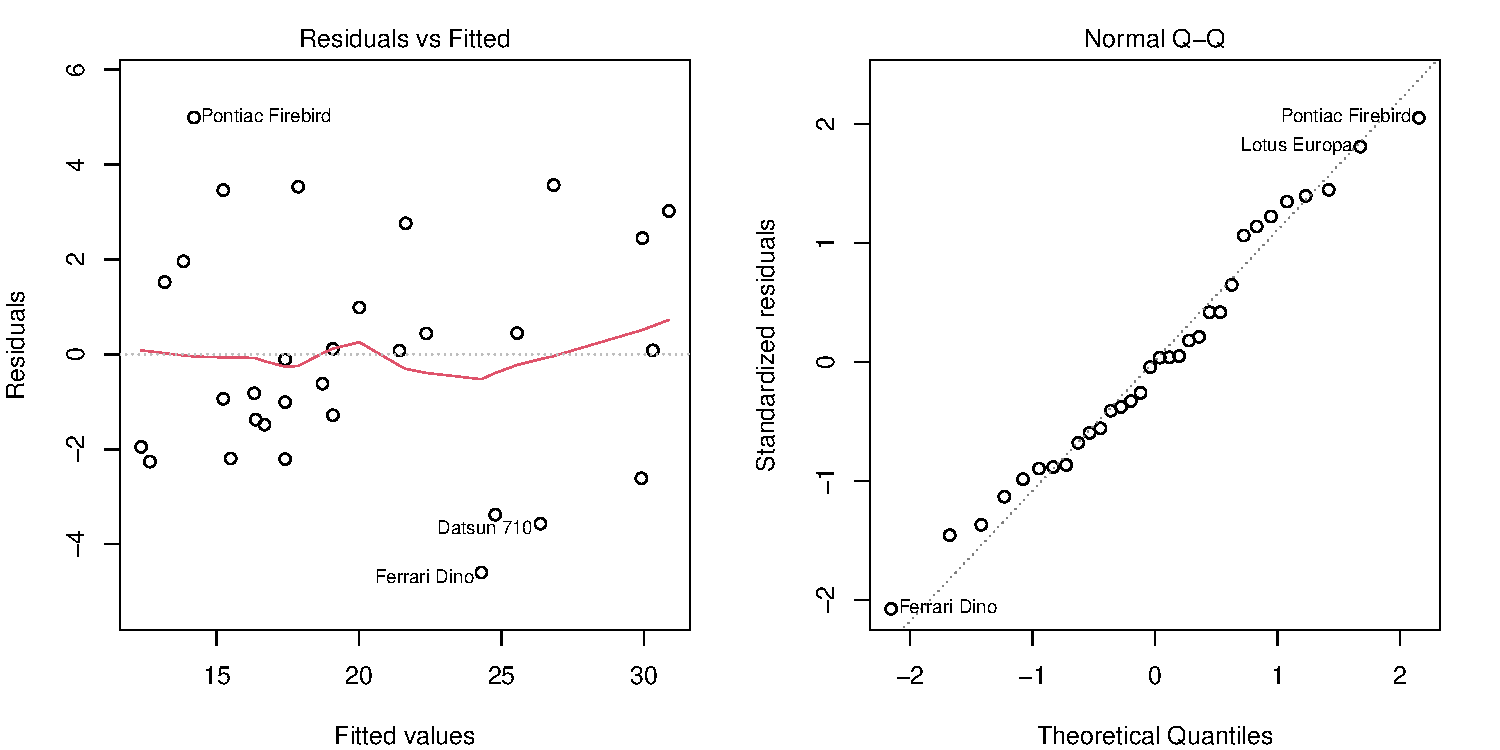
\includegraphics[width=1\linewidth]{03-Lecture_files/figure-beamer/unnamed-chunk-26-1}

\normalsize

\begin{enumerate}[<+->]
\tightlist
\item
  Points in Plot 1 should show \emph{no pattern} (shotgun blast)
\item
  Points in Plot 2 should be \emph{roughly} on top of the 1:1 line
\end{enumerate}
\end{frame}

\begin{frame}[fragile]{Problem 1: Non-linear relationship}
\protect\hypertarget{problem-1-non-linear-relationship}{}
\begin{columns}[T]
\begin{column}{0.48\textwidth}
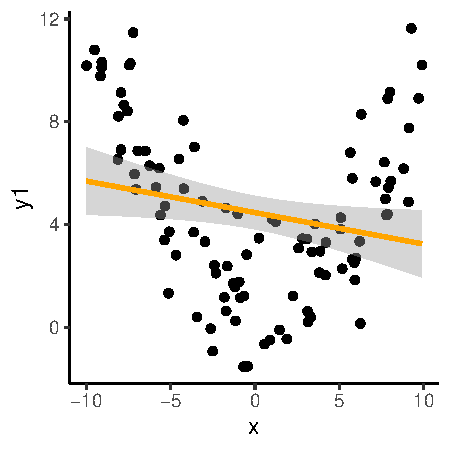
\includegraphics{03-Lecture_files/figure-beamer/unnamed-chunk-27-1.pdf}

\begin{Shaded}
\begin{Highlighting}[]
\FunctionTok{lm}\NormalTok{(y1}\SpecialCharTok{\textasciitilde{}}\NormalTok{x,}\AttributeTok{data=}\NormalTok{d1)}
\end{Highlighting}
\end{Shaded}

\(y1\) clearly follows a hump-shaped relationship, not a linear one
\end{column}

\begin{column}{0.48\textwidth}
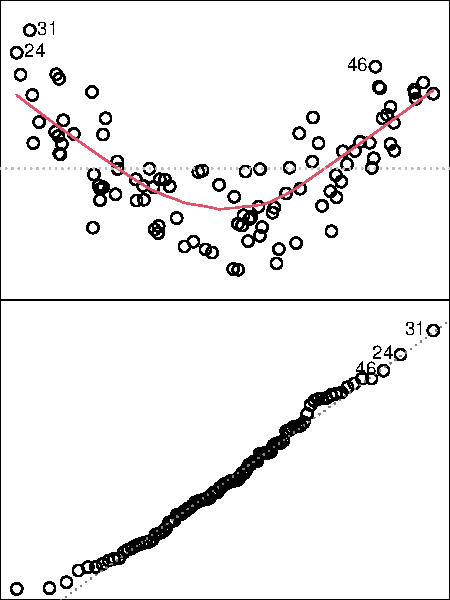
\includegraphics{03-Lecture_files/figure-beamer/unnamed-chunk-29-1.pdf}
\end{column}
\end{columns}
\end{frame}

\begin{frame}[fragile]{Solution: transform predictors}
\protect\hypertarget{solution-transform-predictors}{}
\begin{columns}[T]
\begin{column}{0.48\textwidth}
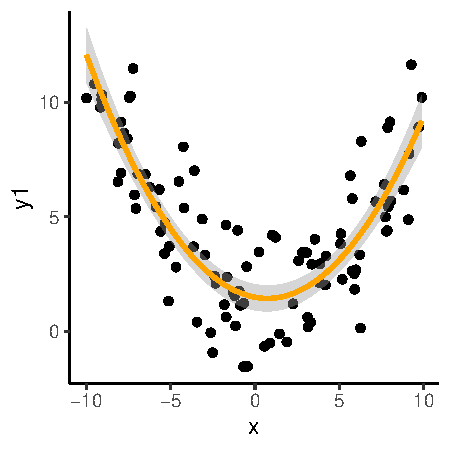
\includegraphics{03-Lecture_files/figure-beamer/unnamed-chunk-30-1.pdf}

\begin{Shaded}
\begin{Highlighting}[]
\FunctionTok{lm}\NormalTok{(y1}\SpecialCharTok{\textasciitilde{}}\FunctionTok{poly}\NormalTok{(x,}\DecValTok{2}\NormalTok{),}\AttributeTok{data=}\NormalTok{d1)}
\end{Highlighting}
\end{Shaded}

\small

\emph{log} and \emph{square-root} transformations are common
\end{column}

\begin{column}{0.48\textwidth}
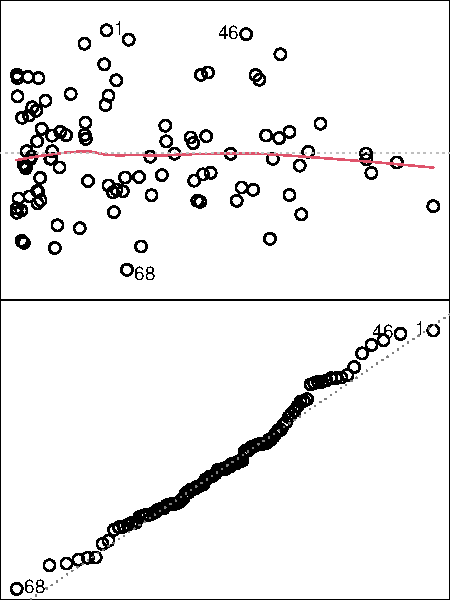
\includegraphics{03-Lecture_files/figure-beamer/unnamed-chunk-32-1.pdf}
\end{column}
\end{columns}

\small

\begin{itemize}[<+->]
\tightlist
\item
  Warning: Polynomials can do weird things; consider whether this is
  biologically reasonable!
\end{itemize}
\end{frame}

\begin{frame}[fragile]{Problem 2a: Non-normal response}
\protect\hypertarget{problem-2a-non-normal-response}{}
\begin{columns}[T]
\begin{column}{0.48\textwidth}
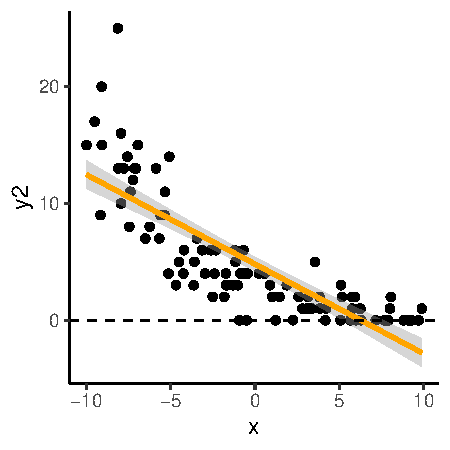
\includegraphics{03-Lecture_files/figure-beamer/unnamed-chunk-33-1.pdf}

\begin{Shaded}
\begin{Highlighting}[]
\FunctionTok{lm}\NormalTok{(y2}\SpecialCharTok{\textasciitilde{}}\NormalTok{x,}\AttributeTok{data=}\NormalTok{d1)}
\end{Highlighting}
\end{Shaded}

\(y2\) is count data (integers \(\geq{0}\)). \emph{Very} common in
ecological data.
\end{column}

\begin{column}{0.48\textwidth}
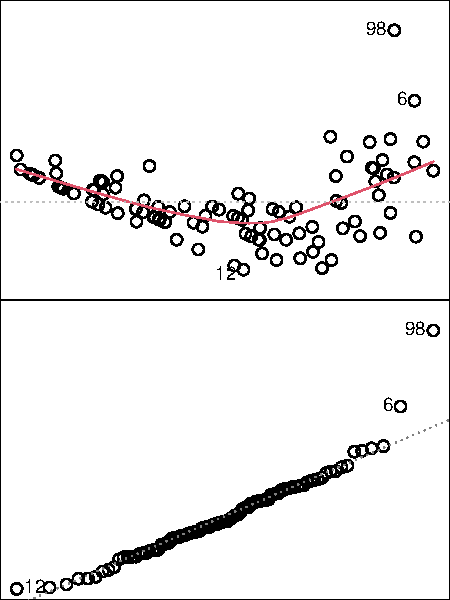
\includegraphics{03-Lecture_files/figure-beamer/unnamed-chunk-35-1.pdf}
\end{column}
\end{columns}
\end{frame}

\begin{frame}[fragile]{Solution: transform data to meet assumptions}
\protect\hypertarget{solution-transform-data-to-meet-assumptions}{}
\begin{columns}[T]
\begin{column}{0.48\textwidth}
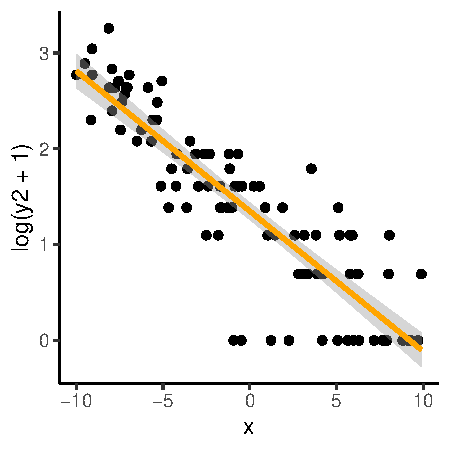
\includegraphics{03-Lecture_files/figure-beamer/unnamed-chunk-36-1.pdf}

\begin{Shaded}
\begin{Highlighting}[]
\FunctionTok{lm}\NormalTok{(}\FunctionTok{log}\NormalTok{(y2}\SpecialCharTok{+}\DecValTok{1}\NormalTok{)}\SpecialCharTok{\textasciitilde{}}\NormalTok{x,}\AttributeTok{data=}\NormalTok{d1)}
\end{Highlighting}
\end{Shaded}

Square-root transformations are also common
\end{column}

\begin{column}{0.48\textwidth}
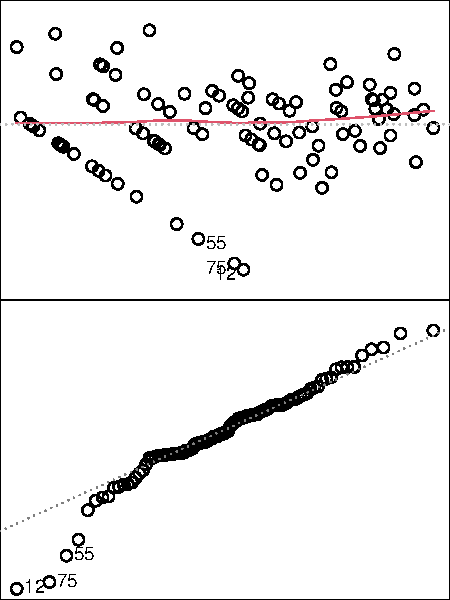
\includegraphics{03-Lecture_files/figure-beamer/unnamed-chunk-38-1.pdf}
\end{column}
\end{columns}
\end{frame}

\begin{frame}[fragile]{Problem 2b: Non-normal response}
\protect\hypertarget{problem-2b-non-normal-response}{}
\begin{columns}[T]
\begin{column}{0.48\textwidth}
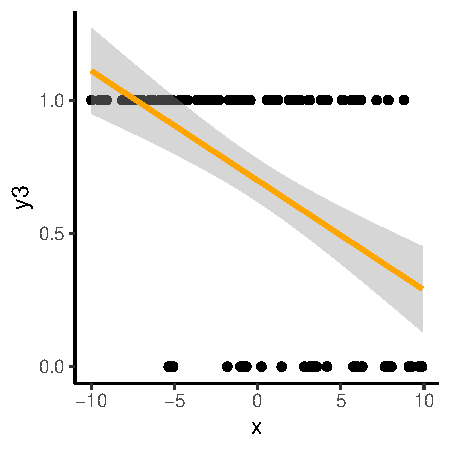
\includegraphics{03-Lecture_files/figure-beamer/unnamed-chunk-39-1.pdf}

\begin{Shaded}
\begin{Highlighting}[]
\FunctionTok{lm}\NormalTok{(y3}\SpecialCharTok{\textasciitilde{}}\NormalTok{x,}\AttributeTok{data=}\NormalTok{d1)}
\end{Highlighting}
\end{Shaded}

\(y3\) is binomial data (success/failure, 0 or 1). \emph{Very} common in
ecological data.
\end{column}

\begin{column}{0.48\textwidth}
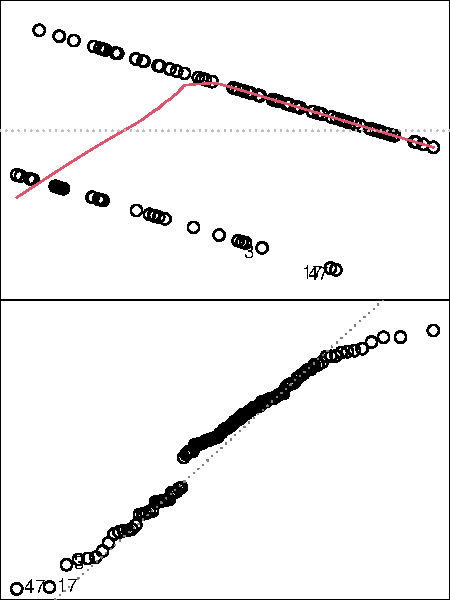
\includegraphics{03-Lecture_files/figure-beamer/unnamed-chunk-41-1.pdf}
\end{column}
\end{columns}
\end{frame}

\begin{frame}{Solution: use a Generalized Linear Model (GLM)}
\protect\hypertarget{solution-use-a-generalized-linear-model-glm}{}
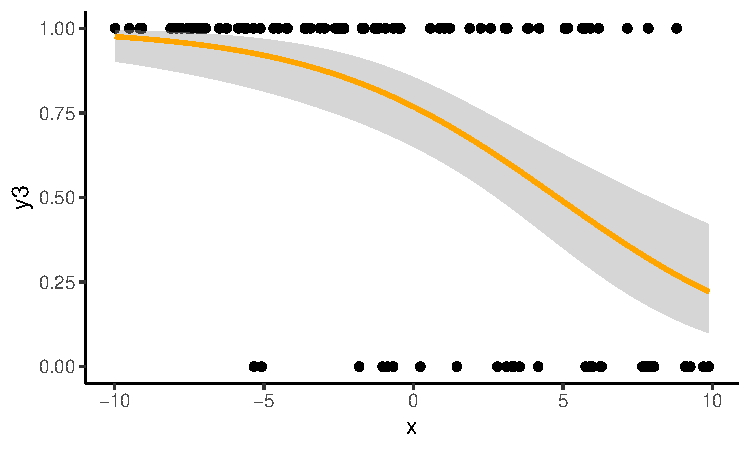
\includegraphics{03-Lecture_files/figure-beamer/unnamed-chunk-42-1.pdf}

\begin{itemize}[<+->]
\tightlist
\item
  This is a topic for another lecture. Hold tight!
\end{itemize}
\end{frame}

\begin{frame}[fragile]{Problem: variables are on different scales}
\protect\hypertarget{problem-variables-are-on-different-scales}{}
\begin{columns}[T]
\begin{column}{0.48\textwidth}
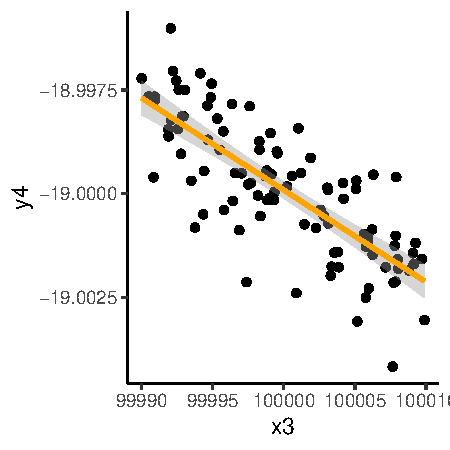
\includegraphics{03-Lecture_files/figure-beamer/unnamed-chunk-43-1.pdf}
\small

\begin{Shaded}
\begin{Highlighting}[]
\FunctionTok{lm}\NormalTok{(y4}\SpecialCharTok{\textasciitilde{}}\NormalTok{x3,}\AttributeTok{data=}\NormalTok{d1)}
\end{Highlighting}
\end{Shaded}

\begin{itemize}[<+->]
\tightlist
\item
  \(y4\) is tiny, while \(x3\) is huge
\item
  OK for now, but can cause problems when fitting complicated models
  (GLMs)
\end{itemize}
\end{column}

\begin{column}{0.48\textwidth}
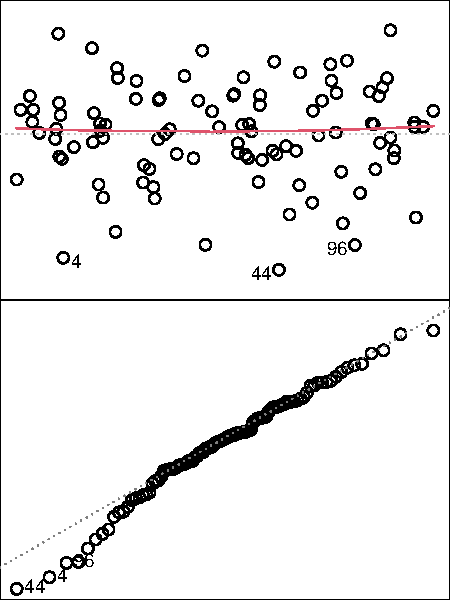
\includegraphics{03-Lecture_files/figure-beamer/unnamed-chunk-45-1.pdf}
\end{column}
\end{columns}
\end{frame}

\begin{frame}[fragile]{Solution: scale data/predictors before fitting}
\protect\hypertarget{solution-scale-datapredictors-before-fitting}{}
\begin{columns}[T]
\begin{column}{0.48\textwidth}
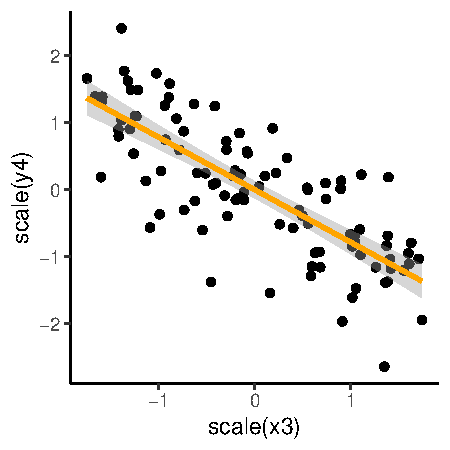
\includegraphics{03-Lecture_files/figure-beamer/unnamed-chunk-46-1.pdf}

\small

\begin{Shaded}
\begin{Highlighting}[]
\CommentTok{\#Subtracts mean, divides by SD}
\NormalTok{d1}\SpecialCharTok{$}\NormalTok{s.y4 }\OtherTok{\textless{}{-}} \FunctionTok{scale}\NormalTok{(y4)}
\NormalTok{d1}\SpecialCharTok{$}\NormalTok{s.x3 }\OtherTok{\textless{}{-}} \FunctionTok{scale}\NormalTok{(x3) }
\FunctionTok{lm}\NormalTok{(s.y4}\SpecialCharTok{\textasciitilde{}}\NormalTok{s.x3,}\AttributeTok{data=}\NormalTok{d1) }\CommentTok{\#Refit}
\end{Highlighting}
\end{Shaded}
\end{column}

\begin{column}{0.48\textwidth}
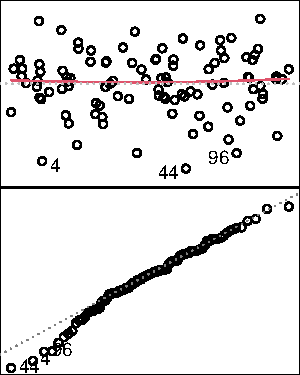
\includegraphics{03-Lecture_files/figure-beamer/unnamed-chunk-48-1.pdf}

\small

\begin{itemize}[<+->]
\tightlist
\item
  Residuals are the same as before
\item
  Coefficients are now related to \emph{scaled} data and predictor
\end{itemize}
\end{column}
\end{columns}
\end{frame}

\begin{frame}[fragile]{But wait\ldots{} there's more (assumptions)!}
\protect\hypertarget{but-wait-theres-more-assumptions}{}
\begin{columns}[T]
\begin{column}{0.48\textwidth}
One more assumption:

\begin{enumerate}[<+->]
\setcounter{enumi}{3}
\tightlist
\item
  If you have 2+ predictors in your model, the predictors are not
  related to each other
\end{enumerate}

\begin{itemize}[<+->]
\tightlist
\item
  Say we have 2 predictors, \(x\) and \(x2\):
\end{itemize}

\begin{Shaded}
\begin{Highlighting}[]
\FunctionTok{lm}\NormalTok{(y0}\SpecialCharTok{\textasciitilde{}}\NormalTok{x}\SpecialCharTok{+}\NormalTok{x2,}\AttributeTok{data=}\NormalTok{d1)}
\end{Highlighting}
\end{Shaded}

\begin{itemize}[<+->]
\tightlist
\item
  Model fits, and residuals look OK, but there's trouble ahead!
\end{itemize}
\end{column}

\begin{column}{0.48\textwidth}
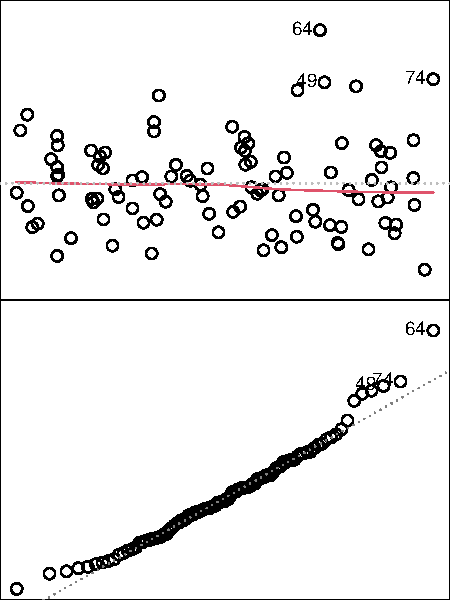
\includegraphics{03-Lecture_files/figure-beamer/unnamed-chunk-50-1.pdf}
\end{column}
\end{columns}
\end{frame}

\begin{frame}[fragile]{Uh oh! Collinearity!}
\protect\hypertarget{uh-oh-collinearity}{}
\begin{columns}[T]
\begin{column}{0.48\textwidth}
\tiny

\begin{Shaded}
\begin{Highlighting}[]
\CommentTok{\#Function to print correlation (r) value}
\NormalTok{corText }\OtherTok{\textless{}{-}} \ControlFlowTok{function}\NormalTok{(x,y)\{}
  \FunctionTok{text}\NormalTok{(}\FloatTok{0.5}\NormalTok{,}\FloatTok{0.5}\NormalTok{,}\FunctionTok{round}\NormalTok{(}\FunctionTok{cor}\NormalTok{(x,y),}\DecValTok{3}\NormalTok{))}
\NormalTok{\} }

\CommentTok{\#Pairplot of y0, x, and x2}
\FunctionTok{pairs}\NormalTok{(d1[,}\FunctionTok{c}\NormalTok{(}\StringTok{\textquotesingle{}y0\textquotesingle{}}\NormalTok{,}\StringTok{\textquotesingle{}x\textquotesingle{}}\NormalTok{,}\StringTok{\textquotesingle{}x2\textquotesingle{}}\NormalTok{)],}\AttributeTok{lower.panel=}\NormalTok{corText)}
\end{Highlighting}
\end{Shaded}

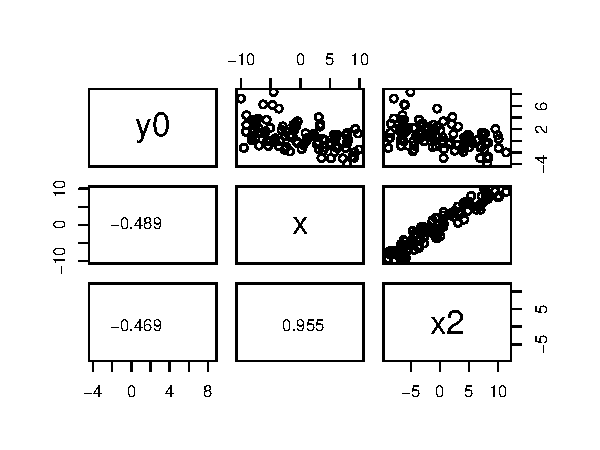
\includegraphics{03-Lecture_files/figure-beamer/unnamed-chunk-51-1.pdf}

\normalsize

\texttt{pairs()} is useful for looking at relations among your data
\end{column}

\begin{column}{0.48\textwidth}
\begin{itemize}[<+->]
\tightlist
\item
  \(x\) and \(x2\) mean basically the same thing!
\item
  Also revealed using variance-inflation factors (VIFs):
\end{itemize}

\small

\begin{Shaded}
\begin{Highlighting}[]
\FunctionTok{library}\NormalTok{(car)}
\CommentTok{\#VIF scores:}
\CommentTok{\# 1 = no problem}
\CommentTok{\# 1{-}5 = some problems}
\CommentTok{\# 5+ = big problems!}
\FunctionTok{vif}\NormalTok{(m2) }
\end{Highlighting}
\end{Shaded}

\begin{verbatim}
##        x       x2 
## 11.31812 11.31812
\end{verbatim}
\end{column}
\end{columns}
\end{frame}

\begin{frame}[fragile]{Is collinearity really that bad?}
\protect\hypertarget{is-collinearity-really-that-bad}{}
\begin{columns}[T]
\begin{column}{0.48\textwidth}
\small

\begin{Shaded}
\begin{Highlighting}[]
\CommentTok{\#Correct model}
\NormalTok{m1 }\OtherTok{\textless{}{-}} \FunctionTok{lm}\NormalTok{(y0}\SpecialCharTok{\textasciitilde{}}\NormalTok{x,}\AttributeTok{data=}\NormalTok{d1)}
\end{Highlighting}
\end{Shaded}

\tiny

\begin{tabular}{l|r|r|r}
\hline
  & Estimate & Std. Error & Pr(>|t|)\\
\hline
(Intercept) & 0.7851936 & 0.1943002 & 0.0001059\\
\hline
\textcolor{red}{x} & \textcolor{red}{-0.1900346} & \textcolor{red}{0.0342596} & \textcolor{red}{0.0000002}\\
\hline
\end{tabular}
\end{column}

\begin{column}{0.48\textwidth}
\small

\begin{Shaded}
\begin{Highlighting}[]
\CommentTok{\#Incorrect model}
\NormalTok{m2 }\OtherTok{\textless{}{-}} \FunctionTok{lm}\NormalTok{(y0}\SpecialCharTok{\textasciitilde{}}\NormalTok{x}\SpecialCharTok{+}\NormalTok{x2,}\AttributeTok{data=}\NormalTok{d1)}
\end{Highlighting}
\end{Shaded}

\tiny

\begin{tabular}{l|r|r|r}
\hline
  & Estimate & Std. Error & Pr(>|t|)\\
\hline
(Intercept) & 0.7860300 & 0.1955770 & 0.0001155\\
\hline
\textcolor{red}{x} & \textcolor{red}{-0.1812556} & \textcolor{red}{0.1158464} & \textcolor{red}{0.1209288}\\
\hline
x2 & -0.0094931 & 0.1196074 & 0.9369028\\
\hline
\end{tabular}
\end{column}
\end{columns}

\begin{itemize}[<+->]
\tightlist
\item
  Increases SE of each term, so model may ``miss'' important terms
\item
  Gets worse with increasing correlation, or if many terms are
  correlated!
\end{itemize}
\end{frame}

\begin{frame}[fragile]{How do we fix this? Depends on your goals:}
\protect\hypertarget{how-do-we-fix-this-depends-on-your-goals}{}
\begin{columns}[T]
\begin{column}{0.48\textwidth}
\begin{enumerate}[<+->]
\tightlist
\item
  I care about predicting things
\end{enumerate}

\begin{itemize}[<+->]
\tightlist
\item
  Use dimensional reduction (e.g.~PCA) and re-run model
\end{itemize}

\begin{enumerate}[<+->]
\setcounter{enumi}{1}
\tightlist
\item
  I care about what's causing things
\end{enumerate}

\begin{itemize}[<+->]
\tightlist
\item
  Design experiment to separate cause and effect
\item
  Think about what is causing what. \emph{Graphical models} are helpful
  for this

  \begin{itemize}[<+->]
  \tightlist
  \item
    Not all variables have to be included!
  \end{itemize}
\end{itemize}
\end{column}

\begin{column}{0.48\textwidth}
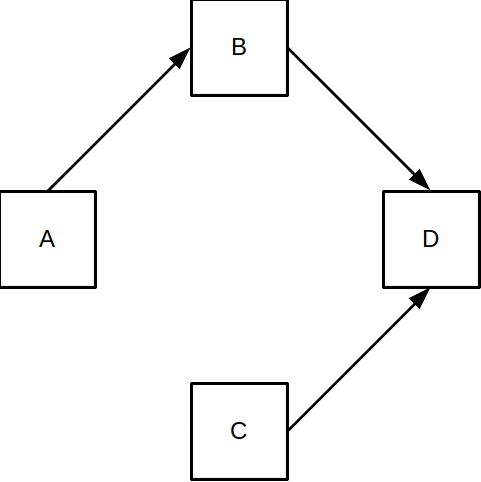
\includegraphics[width=0.8\linewidth]{./dag}

\begin{itemize}[<+->]
\tightlist
\item
  Simple graphical model, where the effect of A on D is \emph{mediated}
  by B.
\item
  ``Correct'' \texttt{lm} model of D:
\end{itemize}

\texttt{lm(D\ \textasciitilde{}\ B\ +\ C)}
\end{column}
\end{columns}
\end{frame}

\begin{frame}[fragile]{A challenger approaches!}
\protect\hypertarget{a-challenger-approaches-2}{}
\begin{itemize}[<+->]
\tightlist
\item
  Guess what\ldots{} more bat data! This time there are 6 variables that
  were measured. We're interested in predicting \texttt{bats} (counts of
  bats per night).
\item
  Formulate a causal model that seems reasonable

  \begin{itemize}[<+->]
  \tightlist
  \item
    Draw it out on paper/in PowerPoint using flow diagrams
  \end{itemize}
\item
  Fit an \texttt{lm} model of \texttt{bats} from your causal model,
  check the assumptions, and update as necessary
\end{itemize}
\end{frame}

\begin{frame}[fragile]{Here's the answer}
\protect\hypertarget{heres-the-answer}{}
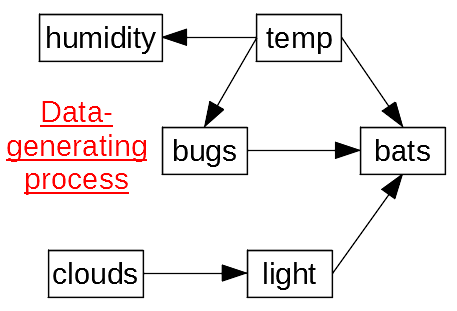
\includegraphics[width=0.7\linewidth]{./dag2}

This is the \textbf{true} process that generated the data. Model for
\texttt{bats} should look like:

\texttt{lm(log(bats+0.1)\textasciitilde{}poly(temp,2)+light+bugs,data=dat)}
\end{frame}

\end{document}
